% \iffalse meta-comment
%<*internal>
\iffalse
%</internal>
%<*readme>
----------------------------------------------------------------
phd-utils --- some useful uitlities
E-mail: yannislaz@gmail.com
Released under the LaTeX Project Public License v1.3c or later
See http://www.latex-project.org/lppl.txt
----------------------------------------------------------------
This file provides a phd for defining a class.
%</readme>
%<*readmemd>
###The `phd` LaTeX2e package

The `phd` latex package and the class with the same name provide
convenient methods to create new styles for books, reports
and articles. It also loads the most commonly used packages 
and resolves conflicts.

This work consists of the file  `phd.dtx`,
and the derived files   `phd.ins`,  `phd.pdf`, and `phd.sty`.

The `phd` bundle is a bunch of 15 packages, that manage all
aspects of document production.

They consist of:

1.0  The [phd-pkgmanager](https://github.com/yannisl/phd/blob/master/docs/phd-pkgmanager.md). This
     package manages all aspects of loading numerous packages and avoiding conflicts. It currently
     loads over 100 packages, directly or indirectly.
     
2.0  The [phd-fontmanager](https://github.com/yannisl/phd/blob/master/docs/phd-fontmanager.md). The
     `phd-fontmanager` sets up the fonts to be used for the document and provides an interface to
     all areas where font data is needed.
     
3.0  The [phd-handlers](https://github.com/yannisl/phd/blob/master/docs/phd-handlers.md). As we use
     extensively automatic key generation via code, this package provides numerous handlers.
     
4.0  The [phd-lowerlevelheadings](https://github.com/yannisl/phd/blob/master/docs/phd-lowerlevelheadings.md)     

5.0  The [phd-toc](https://github.com/yannisl/phd/blob/master/docs/phd-toc.md) package.
     Manages all aspects of Table of Contents via a key value interface. 

6.0  The [phd-counters](https://github.com/yannisl/phd/blob/master/docs/phd-counters.md) 

7.0  The [phd-colorpalette](https://github.com/yannisl/phd/blob/master/docs/phd-colorpalette.md). This
     package introduces the concept of a `color palette` to `LaTeX` coding. It groups all color
     data into `palettes`. By setting a single set of keys, the document can be updated with new
     color information.

8.0  The [phd-scriptsmanager](https://github.com/yannisl/phd/blob/master/docs/phd-scriptsmanager.md).
     Handles the settings and provides a key face interface to over scripts for use in typesetting
     texts from ancient to modern.

9.0  The [phd-documentation](https://github.com/yannisl/phd/blob/master/docs/phd-documentation.md).
     Provides numerous commands and keys for typesetting code. It also provides indexing shortcuts,
     including math symbols etc.
     
10.0 The [phd-epigraphs](https://github.com/yannisl/phd/blob/master/docs/phd-epigraphs.md).
     This package manages the typesetting of epigraphs.
     
11.0 The [phd-frontmatter](https://github.com/yannisl/phd/blob/master/docs/phd-epigraphs.md)
     package for the typesetting of frontmatter such as coverpages, copyright pages and title
     pages.
     
12.0 The [phd-lorems](https://github.com/yannisl/phd/blob/master/docs/phd-lorems.md)    
     package. Provides some additional commands for filler text.

13.0 The [phd-quote](https://github.com/yannisl/phd/blob/master/docs/phd-quote.md)    
     package. Provides some additional commands for filler text.
     
14.0 The [phd-lists](https://github.com/yannisl/phd/blob/master/docs/phd-lists.md)    
     package. Provides some additional commands and a key value interface for lists.  
     
15.0 The [phd-logos](https://github.com/yannisl/phd/blob/master/docs/phd-logos.md)    
     package. Supplementary commands for logos.         
      
###Installation

run
        `phd-lua phd.dtx` on windows
        
If you have any difficulties with the package come and join us at
http://tex.stackexchange.com and post a new question or
add a comment at http://tex.stackexchange.com/a/45023/963.
or send me a message at  yannislaz at gmail.com

### Documentation

The package was written using the `doc` and `docscript` packages,
so that it is self documented in a literary programming style. 
The .pdf is a fat document, providing over fifty book styles (the
equivalent of classes) plus there is a lot of write-up on the inner
workings of TeX and LaTeX2e. However, you don't need to know much
to use it.

      \usepackage{phd}
      \input{style13}

All choices, are made via an extended key-value interface. 
Although not a compliment, it resembles CSS and the keys are a bit verbose but
attributes are easy to change and have a consistent and easy to remember interface.

To set or add a key we only use one command:

      \cxset{chapter name font-size: Huge,
             chapter number font-size: HUGE} 

### Future Development

This is still an experimental version, but I will retain the
interface in future releases. There is a large amount of
work still to be carried out to improve the template styles
provided, to test it more thoroughly and to add a number of
improvements in the special designs. At present I estimate
that I have completed about 70% of the work that needs
to be done.

__The package as it stands is not production stable.__ 


%</readmemd>
%
%<*TODO>
1. On final round add pkg options. This was left as last in order not to solve problems by adding
    options. Too many options are not a good User Interface.
2.  Finish symbol management, both text and math. Math already 60% incorporated.
3.  Better integration of indexing commands.   
4.  Revisit layout manager for Chapters. Broke again in tests.
5.  Docs. Add all references.
6.  Incorporate phd class for more flexibility.
7. Improve package manager.
8. Group script loading for better font management.
9. General font management to relook it again.
10. Add all style sections (about 100 already prepared). Once they
     are all working issue beta version.
%</TODO>
%<*internal>
\fi
\def\nameofplainTeX{plain}
\ifx\fmtname\nameofplainTeX\else
  \expandafter\begingroup
\fi
%</internal>
%<*install>
\input docstrip.tex
\keepsilent
\askforoverwritefalse
\preamble
----------------------------------------------------------------
phd --- A package to beautify documents.
E-mail: yannislaz@gmail.com
Released under the LaTeX Project Public License v1.3c or later
See http://www.latex-project.org/lppl.txt
----------------------------------------------------------------
\endpreamble
%\BaseDirectory{C:/users/admin/my documents/github/phd}
%\usedir{MWE}
\generate{\file{\jobname.sty}{
  \from{\jobname.dtx}{package}
}}
%</install>
%<install>\endbatchfile
%<*internal>
%\usedir{tex/latex/phd}
\generate{
  \file{\jobname.ins}{\from{\jobname.dtx}{install}}
}
\nopreamble\nopostamble

\generate{
	\file{README.txt}{\from{\jobname.dtx}{readme}}
  }

\generate{
  \file{README.md}{\from{\jobname.dtx}{readmemd}}
}
\generate{
  \file{TODO.tex}{\from{\jobname.dtx}{TODO}}
}

\ifx\fmtname\nameofplainTeX
  \expandafter\endbatchfile
\else
  \expandafter\endgroup
\fi
 
\immediate\write18{makeindex -s gglo.ist -g phd.gls phd.glo}  %needs checking from trivfloat
\immediate\write18{makeindex -s gind.ist -g phd.ind phd.idx} %needs checking from Joseph’s trivfloat
%</internal>
%<*driver>
\NeedsTeXFormat{LaTeX2e}[2017/04/15]%
\RequirePackage[2017/04/15]{latexrelease}
\documentclass[twoside,10pt,a4paper]{phddoc}
\usepackage{phdfilecontents}
\def\partname{Part}
\let\HUGE\huge
\usepackage[bottom=2cm]{geometry}
\savegeometry{std}
\usepackage[microtype=on]{phd}
\usepackage{phd-fontmanager}
\usepackage{phd-runningheads}
\usepackage{phd-lowersections}
\usepackage{phd-documentation}
\usepackage{phd-toc}
\sethyperref
\usepackage{makeidx}
\makeindex
\cxset{part format=stewart,
       chapter afterindent=on,
       subsection afterindent=off,
       part afterindent=on,
       section format=hang,
       chapter format=block,
       chapter opening=left}
       
\begin{document}
\DEBUGOFF

\frontmatter
\tableofcontents
%\listoffigures
%\listoftables
\mainmatter
\pagestyle{headings-sugar-hearts}
\parindent1em
%%\makeatletter\@specialtrue\makeatother
%\cxset{custom = stewart}
%\cxset{steward,
%  numbering=arabic,
%  custom=stewart,
%  offsety=0cm,
%  image={./images/hine03.jpg},
%  texti={When Lamport designed the original \LaTeX\ sectioning commands, limitations of computer power forced him to restrict the abstraction of complicated chapter layouts. With current tools available improvements are much easier to program.},
%  textii={In this chapter we discuss a method that allows the production of fancy section headings and formatting, based on a set of key values. Central  to this process is the separation of content from presentation.
%We also discuss the basic formatting tools that are available and how one can modify them to mould new book designs.
% }
% }


\cxset{defaults, chapter format=traditional, 
       chapter opening = left, 
       }


\chapter{Lower Level Headings}


\section{Introduction}

Good book design dictates that sectioning styles follow that the general book design and theme. An academic publication for example might have chapters and section numbered in arabic numerals, whereas a high school textbook might have sections marked in colored boxes. Most traditional books had very humble headings,
set in black ink and the reason was economics. Nowdays most publications will be read online and the use
of color can be useful.

Similarly to the chapter key value interface, the package offers a key value interface to adjust sectioning command parameters.



\cxset{section afterskip={10pt}}

\section{Section styling}

In a similar fashion to the chapter commands the following keys are provided.

\subsection{Fonts and numerals}

Font and numeral keys are shown below.
\medskip
\begin{docKey}[phd]{section font-size}{ = \marg{sizing commands}} {no default, intial=Large}
The font-size command takes arguments
of the  type |Large|, |large| both as commands or without the backslash, which is the recommended way
of setting styles with the |phd| package. 
\end{docKey}

\begin{docKey}[phd] {section font size} {= \marg{sizing commands}} {normal size} 
All the font commands, come in two flavours,
with a hyphen or without, in order to present a user interface that is similar to |pgf/TikZ| conventions for that
are familiar with \latex and another for those used to |CSS| conventions.
\end{docKey}

\begin{docKey}{/phd/section font-family}{= \marg{sizing commands}}{no default, initial value normal} The font-family key, accepts normal LateX values
related to families, but if LuaTeX or XeLaTeX are present it can also accept commands created with |\newfontfamily| 
command of the |fontspec| package, which is loaded automatically by the |phd| package. The package has a database of a number of human friendly names for fonts and commands. If one of these are detected the
family is created at run-time to avoid overloading too many fonts at start-up. 
\begin{verbatim}
\cxset{section font-family = Arial}
\cxset{section font-family = sffamily}
\cxset{section font-family = ttfamily}
\end{verbatim}
The family command family name (if undeined by the user), defaults to the human friendly version name but without the spaces. 
\end{docKey}

%
%  \keyval{section font-weight}{\marg{cmd}}{Font weight command such as \cs{bfseries.}}
%  \keyval{section font-family}{\marg{cmd}}{Font family command such as \cs{sffamily.}}
%  \keyval{section font-shape}{\marg{cmd}}{Font shape command such as \cs{itshape}}
%  \keyval{section color}{\marg{color}}{Color of section.}
%  \keyval{section numbering}{\marg{arabic|roman|Roman|alph|Alph|words|WORDS}}{Section number style.}
  \begin{marglist}
  \item [arabic] Typesers the section number in arabic numerals.
  \item [roman] Typesets the section number in lowercase roman numerals.
  \item [Roman] Typesets the section number in uppercase roman numerals.
  \item [alph] Typesets the section number in lowercase alphabetic numbering.
  \item [Alph] Typesets the section number in uppercase alphabetic numerals.
  \item [words] Typesets the numbers in words (lowercase).
  \item [WORDS] Typesets the number in words (uppercase).
  \end{marglist}

\subsection{Skip and indentation commands}

The keys for indentation and above and below skips are shown below.
\medskip

\keyval{section beforeskip}{}{}
\keyval{section afterskip}{}{}
\keyval{section indent}{\marg{dim}}{Indentation from margin as per standard LaTeX class definitions.}
\keyval{section spaceout}{}{}
\begin{marglist}
 \item[soul]
 \item[none]
\end{marglist}



\subsection{align}

\keyval{section align}{\marg{cmd}}{One of the alignment commands centering, ragged right, raggedleft}

\subsection{Hooks}

Hooks for adding material are shown in the following sketch.
\medskip

\fbox{aboveskip}

\fbox{indent} \fbox{number}\fbox{hook}\fbox{title}

\fbox{belowskip}


\section{Example usage}

In our first example we will use a predefined style for the chapter headings, so we do not need to clutter the example with the chapter commands that we have previously discussed. Our first example will number the section in lower roman, enclosed in brackets and center it.


\makeatletter\@specialfalse
\cxset{
% chapter toc=false,
% chapter  name=CHAPTER,
% numbering=arabic,
% number font-size=huge,
% number font-family=sffamily,
% number font-weight=bfseries,
% number before=,
% number dot=,
% number after=\hspace{1em},
% number position=rightname,
% chapter opening=anywhere,
% chapter font-family=sffamily,
% chapter font-weight=bfseries,
% chapter font-size=huge,
% chapter before={\vspace*{0.1\textheight}\hfill},
% chapter after={\hfill\hfill\vskip0pt\thinrule\par},
% chapter color=black!90,
% number color= black!90,
% title beforeskip={\vspace*{30pt}},
% title afterskip={\vspace*{30pt}\par},
% title before={\hfill},
% title after={\hfill\hfill},
% title font-family=\sffamily,
% title font-color= black!90,
% title font-weight=bfseries,
% title font-size=huge,
 section font-size= LARGE,
 section font-weight= bold,
 section font-family= sffamily,
 section align= centering,
 section numbering=arabic,
 section indent=0em,
 section align= centering,
 section beforeskip=20pt,
 section afterskip=10pt,
 section font-shape= itshape,
}

\cxset{book/.style={
 section numbering=arabic,
 section font-size=Large,
 section font-weight=bfseries,
 section font-family=rmfamily,
 section font-shape=normalfont,
 section align=\raggedright,
 subsection font-size=\large
 section indent=0em,
 section beforeskip=-3.5ex \@plus -1ex\@minus -0.2ex,
 section afterskip=2.3ex\@plus.2ex,
 subsection beforeskip=-3.5ex \@plus -1ex\@minus -0.2ex,
 subsection afterskip= 1.5ex \@plus .2ex,
}}
\makeatother


\begin{texexample}{Adjusting section parameters}{ex:sec}
\cxset{ section font-size= LARGE,
 section font-weight= bold,
 section font-family= sffamily,
 section font-shape=upshape,
 section numbering=(roman), 
 section indent=0em,
 section align= centering,
 section beforeskip=20pt,
 section afterskip=10pt,
 subsection afterskip=3pt,
 subsubsection afterskip=3pt,
 section align=right}
\chapter{A First Look at the Sectioning Keys}
\section{First section}
\lorem
  % adjust counter number so it does not affect the
  % rest of the document
%\addtocounter{section}{-1}
\end{texexample}


The keys are mostly self-explanatory. We have used a |beforeskip| and |afterskip| without any glue. The numbering is just a continuation of the document sections. 

One notable thing to keep in mind is that the numbering of the chapter is independent of that for the section, so if you need to have strange combinations rather define a section numbering custom.\index{section formatting>vertical space}


\cxset{section numbering=arabic}

\subsection{Adjusting vertical spaces}

Perhaps the most important issues we need to consider is the adjusting of vertical spaces; example~\ref{ex:latex}, that follows illustrates settings from the Octavo class and compare them with those of standard the \LaTeXe\ book class. The Octavo class through settings that are based on baselineskip fractions and multiples endeavours to achieve a grid layout. The class also tones down the `loudness' of some of the headings compared to those of the book class.

\makeatletter
\cxset{octavo/.style={
 section font-size=large,
 section font-weight=,
 section font-family=rmfamily,
 section font-shape=scshape,
 section indent=0em,
 section align=\centering,
 section beforeskip=-1.666\baselineskip\@minus -2\p@,
 section afterskip=0.835\baselineskip \@minus 2\p@,
 section after indent = false,
 subsection numbering=none,
 subsection font-family= rmfamily,
 subsection font-size=,
 subsection font-shape=scshape,
 subsection font-weight=,
 subsection indent=1em,
 subsection align=RaggedRight,
 subsection beforeskip=-0.666\baselineskip\@minus -2\p@,
 subsection afterskip=0.333\baselineskip \@minus 2\p@,
 subsection color=spot!50,
 subsubsection color=spot!50,
 }}


\cxset{book/.style={
 section numbering=arabic,
 section font-size= Large,
 section font-weight= bfseries,
 section font-family= rmfamily,
 section font-shape= upshape,
 section align= RaggedRight,
 subsection font-size= large,
 section indent=0em,
 section beforeskip=-3.5ex plus -1ex minus -0.2ex,
 section afterskip=2.3ex plus 0.2ex,
 subsection font-size= large,
 subsection font-weight= bfseries,
 subsection numbering=arabic,
 subsection indent=0pt,
 subsection beforeskip=-3.5ex \@plus -1ex\@minus -0.2ex,
 subsection afterskip= 1.5ex \@plus .2ex,
}}

\cxset{octavo headings/.style={
 section numbering=none,
 section font-size=Large,
 section font-weight=,
 section font-family=rmfamily, section font-shape= scshape,
 section indent=0em, 
 section align=centering, 
 section afterindent=off,
 section beforeskip=-1.666\baselineskip\@minus -2\p@,
 section afterskip=0.835\baselineskip \@minus 2\p@, 
 %
 subsection numbering=none,
 subsection font-family=\rmfamily, 
 subsection font-size=, subsection font-shape=scshape,
 subsection font-weight=, subsection indent=1em, 
 subsection align= RaggedRight,
 subsection beforeskip=-0.666\baselineskip\@minus -2\p@,
 subsection afterskip=0.333\baselineskip \@minus 2\p@,
 subsubsection numbering=none,
 subsubsection font-family= rmfamily,
 subsubsection font-size=,
 subsubsection font-shape= itshape,
 subsubsection font-weight=,
 subsubsection indent = 0em,
 subsubsection align= raggedright,
 subsubsection beforeskip= 0.666\baselineskip\@minus -.2\p@,
 subsubsection afterskip= 3pt, %1.5\baselineskip \@minus .2\p@,
 subsubsection color=spot!50,
 paragraph numbering=none,
 paragraph font-family= rmfamily,
 paragraph font-size=,
 paragraph font-shape=itfamily,
 paragraph font-weight=,
 paragraph color = spot!50,
 paragraph indent=0em,
 paragraph align= RaggedRight,
 paragraph beforeskip=10pt,
 paragraph afterskip=1em,
}}
\makeatother

%\cxset{octavo headings}


%\begin{texexample}{Octavo class headings, settings}{}
%\cxset{octavo headings/.style={
% section numbering=none,section font-size=large,
%section font-weight=,
% section font-family=rmfamily, section font-shape=scshape,
% section indent=0em, 
% paragraph numbering=none,
% paragraph font-family=rmfamily,
% paragraph font-size=,
% paragraph font-shape=,
% paragraph font-weight=,
% paragraph indent=-1em,
% paragraph align=raggedright,
% paragraph beforeskip= 0pt,
% paragraph afterskip=0pt,
%}}
%
%\cxset{octavo headings}
%\renewsection\renewsubsection\renewsubsubsection
%\section{Octavo Class Heading}
%\lorem
%\subsection{Octavo subsection}
%This is some text short text\par
%\subsubsection{Octavo sub-subsection}
%\lorem
%\paragraph{paragraph heading} This is some short text.
%\makeatother
%\end{texexample}

\begin{comment}
The following example was set using the |style| |\cxset{Octavo headings}| with some minor adaptations to enable us to show it inline with the rest of the material on this page\footnote{We set it using \cs{cxset}\marg{chapter opening = anywhere}}. We kept the use of a typical colour throughout the text, whereas the Octavo class, does not allow the use of color.

\cxset{chapter opening = anywhere,
          chapter color = spot!50,
          title font-color = spot!50,
          chapter name={},
          chapter numbering = none,
          chapter before = \addvspace{\baselineskip},
          chapter after = ,
          title spaceout=soul,
          title before =,
          title afterskip=\bigskip\bigskip,
          number before=,
          number after=,
          }
          
\bgroup
\parindent=0pt
\par

\chapter{Octavo Chapter Heading}
\lorem

\section{Octavo Class Heading (Section) }
\lorem

\subsection{Octavo subsection}
\lorem

\subsubsection{Octavo sub-subsection}
\lorem

\paragraph{Paragraph heading} This is some short text.
\lorem

\paragraph{paragraph heading} This is some short text.
\lorem

\egroup
\end{comment}

\begin{texexample}{\LaTeXe\ book class headings settings}{ex:latex}
\makeatletter
\bgroup
\cxset{book/.style={
 section number prefix = \thechapter.,
 section numbering=Roman,
 section number after=,
 section font-size= Large,
 section font-weight=bfseries,
 section font-family=rmfamily,
 section font-shape=upshape,
 section align=RaggedRight,
 section beforeskip=10pt,
 section spaceout = none,
 section color  = red,
 subsection font-size=large,
 section indent=0em,
 section beforeskip=-3.5ex plus1ex minus0.2ex,
 section afterskip=2.3ex\@plus.2ex,
 subsection color = blue,
 subsection font-size=large,
 subsection font-shape=upshape,
 subsection font-weight=bfseries,
 subsection number prefix=\thesection.,
 subsection numbering = arabic,
 subsection beforeskip=-3.5ex \@plus -1ex\@minus -0.2ex,
 subsection indent= 0pt,
 subsection afterskip= 1.5ex \@plus .2ex,
 subsubsection color=black,
}}

\cxset{book}


\section{LaTeX Book  Class Heading}
\lorem
\subsection{A subsection}
\lorem
\subsubsection{A subsubsection}
\egroup

\makeatother
\end{texexample}



\section{Grid example}

One problem sometimes is that the sectioning commands create problems with grid layouts. Example~\ref{ex:grid} shows example settings.

\begin{texexample}{Section styles from the grid package}{ex:grid}
\makeatletter
\cxset{grid/.style={
 section numbering=arabic,
 section font-size=,
 section font-weight=bfseries,
 section font-family=rmfamily,
 section font-shape=upshape,
 section beforeskip=-.999\baselineskip,
 section afterskip=0.001\baselineskip,
 section align= RaggedRight,
 subsection font-size=,
 section indent=0em,
 subsection font-shape=,
 subsection font-weight=bfseries,
 subsection numbering=arabic,
 subsection indent=0pt,
 subsection beforeskip=1\baselineskip,
 subsection afterskip= -.35\baselineskip,
 subsubsection font-shape=itshape,
 subsubsection font-weight=bfseries,
 subsubsection numbering= roman,
 subsubsection number prefix = (,
 subsubsection number suffix =),
 subsubsection indent=0pt,
 subsubsection beforeskip=1\baselineskip,
 subsubsection afterskip= 3pt, %1\baselineskip,
}}
\cxset{grid}




\begin{multicols}{2}
\section{Grid  Class Heading}
\lorem
\subsection{Grid  subsection.}
\lorem
\subsubsection{A subsubsection heading.}
\lorem
\subsubsection{Another subsection heading.}
\lorem
\end{multicols}
\makeatother
\end{texexample}



The key \option{\bfseries section numbering custom}=\marg{code} is quite powerfull and can be used to define any type of section number style. Just remember that the numbering so far depends on two counters, the \docCounter{c@chapter} and \docCounter{c@section}. What the section numbering does, it redefines the macro \docAuxCommand{thesection} to the new definition provided as argument for the key.

Although the temptation to define a lot of key combinations one would rather define new styles as a more user friendly approach.

\cxset{section numbering=arabic, section align= RaggedRight, section font-shape=upshape, section font-family=rmfamily}

\section{Handling Other Section Levels}

Other sectioning commands such as \cs{subsubsection}, \cs{paragraph} and \cs{subparagraph} have equivalent keys. Examples can be found in the chapters that follow for specific styles.

\section{Technical discussion}

The standard LaTeX classes, book report and article have sections showing dot leaders, whereas in the article class the sections are shown without the dotted lines, as the |\l@section| macro is redefined for articles. With the \pkgname{phd} the distinction is unecessary and style files can do the trick that is, either load style article or book or for that matter any other style that has the relevant settings.

\index{macros!\textbackslash @seccntformat}

\subsection{Lower Section Headings}

\LaTeXe\ offers two pathways in redefining section commands, the first one is \refCom{@startsection} and the second is \refCom{@seccntformat} \index{sectioning macros}. It also uses the macro \cs{secdef} to create the starred and unstarred versions of the sectioning commands.

 In the article document class the entry in the table of contents
 for sections looks much like the chapter entries for the report
 and book document classes.
\begin{tcolorbox}{}
\begin{lstlisting}
% \begin{macro}{\l@section}

%
%    First we make sure that if a pagebreak should occur, it occurs
%    \emph{before} this entry. Also a little whitespace is added and a
\newcommand*\l@section[2]{%
  \ifnum \c@tocdepth >\z@
    \addpenalty\@secpenalty
    \addvspace{1.0em \@plus\p@}%
%    \end{macrocode}
%
%    The macro |\numberline| requires that the width of the box that
%    holds the part number is stored in \LaTeX's scratch register
%    |\@tempdima|. Therefore we put it there. We begin a group, and
%    change some of the paragraph parameters (see also the remark at
%    \cs{l@part} regarding \cs{rightskip}).
%    \begin{macrocode}
    \setlength\@tempdima{1.5em}%
    \begingroup
      \parindent \z@ \rightskip \@pnumwidth
      \parfillskip -\@pnumwidth
%    \end{macrocode}
%    Then we leave vertical mode and switch to a bold font.
%    \begin{macrocode}
      \leavevmode \bfseries
%    \end{macrocode}
%    Because we do not use |\numberline| here, we have do some fine
%    tuning `by hand', before we can set the entry. We discourage but
%    not disallow a pagebreak immediately after a section entry.
%    \begin{macrocode}
      \advance\leftskip\@tempdima
      \hskip -\leftskip
      #1\nobreak\hfil \nobreak\hb@xt@\@pnumwidth{\hss #2}\par
    \endgroup
  \fi}
%</article>
\end{lstlisting}
\end{tcolorbox}



As you can see the dot leaders are not present in the above definition. Although we can get rid of dot leaders in other section by redefining them, it is not as easy to add them back.

As our aim is to be able to have all the classes used a common denominator we can define a command as follows (using book as a base)

\begin{tcolorbox}{}
\begin{lstlisting}
\def\articlesection{
\newcommand*\l@section[2]{%
  \ifnum \c@tocdepth >\z@
    \addpenalty\@secpenalty
    \addvspace{1.0em \@plus\p@}%
    \setlength\@tempdima{1.5em}%
    \begingroup
      \parindent \z@ \rightskip \@pnumwidth
      \parfillskip -\@pnumwidth
      \leavevmode \bfseries
      \advance\leftskip\@tempdima
      \hskip -\leftskip
      #1\nobreak\hfil \nobreak\hb@xt@\@pnumwidth{\hss #2}\par
    \endgroup
  \fi}
}
\end{lstlisting}
\end{tcolorbox}


\begin{docCommand}{@startsection}{}
The \cs{@startdsection} macro is one of those locomotive type of commands. It takes 7 required arguments and 2 optional ones and hidden within it are two booleans. The full set looks like this:

\cs{@startsection} \marg{name} \marg{level} \marg{indent} \marg{beforeskip} \marg{afterskip} \marg{style}[*]
  [\marg{altheading}]\marg{heading}.
\end{docCommand}

\begin{marglist}
\item[name] The name of the level command.
\item [level] A number denoting the depth of the section, chapter=1, section=2, etc. A section number will be printed only if \marg{level} is equal or smaller than the value of \textit{secnumdepth}
\item[indent] The indentation of the heading from the left margin.
\item[beforeskip]  The absolute value of this argument is the skip to leave above the heading. If it is negative, then the paragraph indent of the text following the heading is suppressed.
\item [afterskip] If positive, it is the skip to leave below the heading, else it is the skip to the right of a run-in heading.
\item [style] Sets the style of the heading.
\item[\textup{[*]}] When this is missing the heading is numbered and the corresponding counter is incremented.
\item[\textup{[\textit{altheading}]}] Gives an alternative heading to use in the table of contents and in the running heads. This should be present when the * form is used.
\item[heading] The heading of the new section.
\end{marglist}

%\begin{texexample}{Example formatting run-in section}{}
%\makeatletter
%\bgroup
%\renewcommand\section{
%    \@startsection{section}
%    {1}
%    {0em}
%    {-0.8em}
%    {-0.5em}
%    {\large\normalfont\scshape}}
%\makeatother
%\section[]{test}
%\lorem
%\egroup
%\end{texexample}



Note we run the example in a group so that we will not influence the formatting of this document.

As mentioned earlier there is an additional way to introduce formatting for sections and this is using the command \cs{@seccntformat}, which is responsible for typesetting the counter part of a section title. The default definition of the command typesets the \cs{the} representation of the section counter.

%\begin{texexample}{}{}
%\bgroup
%\renewcommand\section{%
%    \@startsection{section}%
%    {1}%
%    {0em}%
%    {-0.8em}%
%    {-0.5em}%
%    {\large\normalfont\scshape}}
%\renewcommand\@seccntformat[1]{\fbox
%{\csname the#1\endcsname}\hspace{0.5em}}
%\makeatother
%\section[]{test}\label{sec:ok}
%\lorem
%
%See section \ref{sec:ok}.
%\egroup
%\end{texexample}



\cxset{section color=spot!50,
          subsection color = spot!50 }
          
\section{Custom headings}

\begin{docCommand*}{@secdef}{\marg{star command} \marg{unstar command}}
So far we have used the |phd|’s keys to set keys that are affecting the standard commands used by
\latexe to set headings. Another way to achieve this,  is to use the macro
 \cs{@secdef}. Therefore, if you wish to use different definitions of \cs{@seccntformat}
for different headings, you must put the appropriate code into every heading
definition.
\end{docCommand*}



\begin{teXXX}
\newcommand\part{\secdef\starcmd\unstarcmd}
\end{teXXX}

The |part| and |chapter| and sometimes |appendix| are defined this way, but nothing stops us from doing the same for other sectioning commands. What the \cs{secdef} command does it will produce the definitions required for a star or unstarred version of the sectioning command, such as |\section|.\footnote{See \ttfamily File F: ltsect.dtx Date: 2014/09/29 Version v1.0z 360} 

\begin{texexample}{}{}
\bgroup
\makeatletter
\renewcommand\section[2] [?]{%
    \refstepcounter{section}
    \addcontentsline{toc}{section}
    {\protect\numberline{section-\thesection}#1}
    {\raggedright\large\bfseries SECTION-\thesection\par \centering#2\par}
    \sectionmark{#1}
    \@afterheading 
   \addvspace{\baselineskip}
 }%
\section[test]{Section Heading}
\lorem
\makeatother
\egroup
\end{texexample}

Many other strategies can also be implemented that are perhaps easier to grasp.

\begin{teX}
\def\@seccntformat##1{\csname the##1\endcsname{}}
\end{teX}

\begin{comment}
\begin{texexample}{}{}
\makeatletter
\bgroup
\def\strut{\vrule height12pt depth1pt width0pt}
  \renewcommand\section[2] []{% % Complex form:
  \refstepcounter{section}% % step counter/ set label
  \addcontentsline{toc}{section}% % generate toc entry
  {\protect\numberline{\thesection} }%
  {\raggedright\large\bfseries\scshape %
  \parbox[b]{\dimexpr(\linewidth-0.5\columnsep)}{\colorbox{brown!80}%
  {{\vbox{\strut\raise2pt\hbox{#2}}}}}}\vskip0pt% % and number
  \sectionmark{#1}% % add to running header
  \@afterheading % prepare indentation handling
  \vspace{\dimexpr\baselineskip+6pt}%must have a parameter
}
\chapter{Fossil Insects}
\begin{multicols*}{2}\raggedcolumns
\section[Insect Fossilization]{\raggedright \thinspace Insect Fossilization}
\lipsum[1]
\end{multicols*}
\egroup
\makeatother
\end{texexample}
\end{comment}

Of course some work is needed to center the text properly in the middle of the colour box. For all practical purposes it is lining up as per the sample.

In Chapter we discussed a forward, but this may not apply if there are no chapters or we need to treat these as sections, the example \ref{ex:forwardsection} shows such a method.


\begin{texexample}{Defining a Foreward Section}{ex:forwardsection}
\makeatletter
\newcommand\prematter@sp[1]{
\addcontentsline{toc}{section}
{\protect\numberline{}#1}
\sectionmark{#1}
{\LARGE\centering\normalfont\sffamily\colorbox{brown!80}{ \textsc{#1}}\par}%
\@afterheading
\addvspace{\baselineskip}
\@afterindentfalse
}

\newenvironment{prematter}[1]{%
   \prematter@sp{#1}}
{}
\begin{multicols}{2}
\label{theok}
\begin{prematter}{Foreward}
\lipsum[1]
\end{prematter}\ref{theok}
\end{multicols}
\makeatother
\end{texexample}


\section{underlining}

I am aware that some people have no choice but have some sections underlined as dictated by archaic regulations in some establishments for thesis submission. If nobody is forcing you to underline it is best to avoid it. We use Donald Arsenau's ulem package to achieve underlining. \footnote{\protect\url{http://tex.stackexchange.com/questions/52998/change-title-to-small-caps-but-not-in-toc}}
\endinput

\makeatletter
\gdef\sectionopen{}
\def\@sectionsuffix{}
\def\@sectionprefix{\sectionname\space}
\newif\if@sectioncase \@sectioncasefalse

\cxset{
  section special/.code =\def\specialsection@cx{#1},
  section xcolor/.store in = \sectionxcolor@cx,
  section opening/.is choice,
  section opening/openany/.code=\gdef\sectionopen{\clearpage},
  section opening/right/.code = \gdef\sectionopen{\cleardoublepage},
  section opening/none/.code = \gdef\sectionopen{},
  section top rule/.is choice, 
  section top rule/true/.code =\DeclareRobustCommand\sectiontoprule{%
        \leavevmode\par\noindent\rule{\textwidth}{1pt}\vskip3.5pt},
  section top rule/true/.code=\def\sectiontoprule{\leavevmode\par\noindent\tikzrule},      
  section top rule/false/.code=\gdef\sectiontoprule{},
  % bottom rule
  section bottom rule/.is choice, 
  section bottom rule/true/.code =\DeclareRobustCommand\sectionbottomrule{%
        \leavevmode\par\noindent\rule{\textwidth}{1pt}\vskip.5pt},
  section bottom rule/true/.code=\def\sectionbottomrule{\vskip-0.5\baselineskip\rlap{\tikzrule}},      
  section bottom rule/false/.code=\gdef\sectionbottomrule{},
  % upper and lower case - TODO in lua
  section case/.is choice,
  section case/lower/.code=\def\sectioncase@cx{\@sectioncasetrue
                             \if@sectioncase\expandafter\MakeTextLowercase\fi},
  section  case/upper/.code=\def\sectioncase@cx{\@sectioncasefalse
                    \if@sectioncase\else\expandafter\MakeTextUppercase \fi},
  section  case/none/.code=\def\sectioncase@cx{\@empty},
}
\cxset{
          section special = sectionspecialruled@cx,
          section xcolor=spot!50,
          section afterindent=false,
          section opening=right,
          section top rule=true,
          section bottom rule=true,
          section afterskip=20pt,
          section case=lower,
          section font-family=aegean
          }


%\def\specialsection@cx{sectionspecialruled@cx}
\def\secdef#1#2{\@ifstar{\@dblarg{#2}}{\@dblarg{#1}}}
%
\newcommand\sectionx{%
  \par  
  \sectionopen   %determines if it is to be treated like a chapter
  \addpenalty\@secpenalty\nobreak
  \secdef\sectionspecialruled@cx\@ssection
   } 
  

% The macro sectionspecial@cx is a more generic macro that typesets the block of tex
% for the section heading.
% 
\def\sectionspecialruled@cx[#1]#2{%
   \sectiontoprule
  \ifnum\c@secnumdepth>0\relax
     \refstepcounter{section}%
     \addcontentsline{toc}{section}{%
      \@sectionprefix\thesection\@sectionsuffix
       \texorpdfstring{\quad}{ }#1}%
  \else
     \addcontentsline{toc}{section}{#1}%
  \fi
  {% start the title
    \color{\sectionxcolor@cx}%
    \noindent\centering\interlinepenalty\@M
   \setfont@cx{\sectionfontweight@cx}%
       {\sectionfontfamily@cx}{\sectionfontsize@cx}{\sectionfontshape@cx}%
     \ifnum\c@secnumdepth>0\relax
        \@sectionprefix\thesection\@sectionsuffix
        \quad\sectioncase@cx{#2}%
    \else %
       \sectioncase@cx{#2}
      % \luadirect{tex.print(string.upper(#2))}%
   \fi%
   \sectionbottomrule
   %\expandafter\addvspace\sectionafterskip@cx\relax%
%   \tikzrule 
   %\rule{\textwidth}{3pt}%
   \afterindent@cx
   \nobreak\par}}


\def\@ssection[#1]#2{%
  \phantomsection
  \addcontentsline{toc}{section}{#1}%
  {\noindent\centering\interlinepenalty\@M
   \color{\sectioncolor@cx}
     \setfont@cx{\sectionfontweight@cx}%
       {\sectionfontfamily@cx}{\sectionfontsize@cx}{\sectionfontshape@cx}%
       \sectiontoprule
       
        \sectioncase@cx{#2}%
        \sectionbottomrule
       %\expandafter \addvspace\sectionafterskip@cx \relax
      \afterindent@cx
   \nobreak\par}}
\makeatother

\let\section\sectionx

\section{Special Sections}

When we described the usage of the chapter setting keys, we extended the system to describe commands
for specially constructed chapter heads that do not follow the normal style of \latexe.

This section describes how to design and program, sectioning styles that go a little bit more than those that
can be defined so far and that they will require you to have a bit more knowledge of \tex and \latexe programming skills.

For example, the heading of this section started on a new page and has rules above and below the title and section number. In addition the title was capitalized automatically, despite having been typed as:

\begin{verbatim}
\section{Special Sections}
\end{verbatim}

By setting the key and calling the section again, we can typeset it on the same page

\begin{verbatim}
   \cxset{section opening=none}
   \section{Another example}
\end{verbatim}

\cxset{section opening=none,
          section case=upper,
          section top rule=false,
          section bottom rule=true,
          section afterindent=false}
          
\section{Another example}

Special sections have their own user provided macros, that have been pre-defined by the user and are invoked using the key |section special|. In the example below we have predefined a macro |\sectionsspecialruled@cx|.
Do not use a command in the value just the literal name of the command as shown below,

\begin{verbatim}
\cxset{section special = ruled,}
\end{verbatim}

\cxset{section opening=none,
          section case=none,
          section top rule=true,
          section bottom rule=false}
          
The star section of the command omits the section number from the heading. It will still insert an entry into the toc. If it is provided with an optional argument it will insert the optional text into the toc.

Check the Table of Contents to see the rendering.

\begin{verbatim}
\section*{No number test}
\section*[Short Title]{No number test}
\end{verbatim}

\section*{No number test}
\lorem

\cxset{section bottom rule=true,
         section afterindent=false,
         section font-family=agean}

\section*[Short Title]{No number test}

\lorem

\cxset{chapter opening=any,
          chapter toc=true,
          chapter numbering=arabic}

One can extend these \emph{specials} to much more complicated sections (which can resemble) chapter openings.
\makeatletter 
\newif\if@debug \@debugtrue
\bgroup
\leftskip-3cm \rightskip2cm
\def\hook{\node[right=5pt, yshift=-12pt] at (0,-3) {\HUGE\color{purple} This is the  Title}; }
\def\hook{}

\cxset{chapter name = CHAPTER}
%\expandafter\ifnum\thechapter=0\stepcounter{chapter}\else\fi

\hspace*{-2cm}\begin{tikzpicture}
\if@debug\draw [help lines] (0,0) grid (18,-13);\else\fi
\draw[fill=red]  (0,0) circle (1.5pt) ;
\node[rectangle,draw, right, baseline] (x) at (0,1) {\LARGE\color{black!30}{before}\relax};
\draw[fill=red]  (0,1) circle (1.5pt) ;
\node[rectangle,draw, right=1sp] at (0,0) {\LARGE\color{black!20} \so\chaptername\relax};

\node[rectangle,draw, color=white, below right, fill=blue!50, text=white] at +(\textwidth,0) {\scalebox{2}{\HUGE \thechapter}};
\draw[fill=red]  (0,-3) circle (1.5pt) ;
% The title of the block
\node[rectangle, draw, text width=9cm,below right, yshift=-1pt] at (0,-3) {%
         \sffamily
         \HUGE Title Format\vskip1sp \medskip\Large Blue colors in jeans, dresses skirts\\ and hats.\\
         How to dress in stylish blues. \\Getting your partner to get\\ into LaTeX. }; 
\node at (12.5,-9) {\includegraphics[width=7cm]{./images/fashion.jpg}};
\hook
\end{tikzpicture}
\makeatother
\tikzrule 
\egroup 

For such complex layouts, it is always best to start from a piece of paper where you roughly outline
the design of the template. I call such layouts templates, because we will insert a number of variables
to parameterize them. All the typesetting commands will need to be inserted in a macro, which you
should give it a unique name. We will name the above template \emph{fashion} and we will later on define
a macro \cmd{\fashion}. The sectioning mechanism provided by the \pkgname{phd} will enable the
setting of such layouts to be carried out as:

\begin{verbatim}
\cxset{section custom = fashion}
\end{verbatim}

Everytime we call the above in our document settings, in the preamble or elswehere or subsequent sections will
be typeset using this format. 

Also before you get into too much detail in programming you should define the \emph{new} parameters
that may have to be introduced. In the example above most of the fields are already defined either
using the |phd|  key value interface or by LaTeX itself. What is new here is only the introduction of an image
and perhaps some rules as to its exact location. For example you can establish a rule that if half the width of
the image is less than the right margin then it should be centered at the right side of the textblock, alternatively it should be lined at the end of the page. We will see how to achieve this a bit later on.

It is also best to start with a MWE and to first achieve the layout you want without any parameters being introduced. We assume that we will be using TikZ to position the text and the image exactly where we 
want them, although nothing stops us from using either plain TeX boxes or the picture environment.
Since we are loading the TikZ package it is best though to use it for the graphical layout.

Introduce a |debug| boolean to help you with switching grid lines on and off. Depending on what you are trying to accomplish you may want to also add some hooks into the definitions. Start from the layout first.

\begin{verbatim}
\begin{tikzpicture}
\if@debug
   \draw [help lines] (0,0) grid (18,-13);
\else
\fi
...
\fashionposthook
\end{tikzpicture}
\end{verbatim}

We draw a grid of $18\times13$ cells which just happens to suit this particular layout well; The command 
\cmd{\fashionposthook} was just added to provide any further tikz instructions at runtime.

We then draw the layout first as best as we can and without too much consideration for parameterizing the layout at this stage.

\emphasis{if@debug,else,fi}
\begin{scriptexample}{}{}
\begin{teX}
\begin{tikzpicture}
\if@debug
  \draw [help lines] (0,0) grid (18,-13);
  \draw[fill=red]  (0,0) circle (1.5pt) ;
  \draw[fill=red]  (0,-3) circle (1.5pt) ;
\else
\fi
% draw debug rectangles
\node[rectangle,draw, right, baseline] (x) at (0,1) {\LARGE\color{black!30}{before}\relax};
\draw[fill=red]  (0,1) circle (1.5pt) ;
\node[rectangle,draw, right=1sp] at (0,0) {\LARGE\color{black!20} \so\chaptername\relax};

\node[rectangle,draw, color=white, below right, fill=blue!50, text=white] at +(\textwidth,0) {\scalebox{2}{\HUGE \thechapter}};

% The title of the block
\node[rectangle, draw, text width=9cm,below right, yshift=-1pt] at (0,-3) {%
         \sffamily
         \HUGE Title Format\vskip1sp \medskip\Large Blue colors in jeans, dresses skirts\\ and hats.\\
         How to dress in stylish blues. \\Getting your partner to get\\ into LaTeX. }; 
   \IfFileExists{\fashionimage@cx}%   
         {\node at (12.5,-9) {\includegraphics[width=7cm]{fashion}};}
         { \node at (12.5,-9) {\includegraphics[width=7cm]{fashion}};}
\hook
\end{tikzpicture}
\end{teX}
\end{scriptexample}

As I mentioned earlier, adding parameters increases the complexity of the layout and it might onfuse you
at first, but we do need to go back and iterate to improve the template.

\begin{description}
\item [odd or even pages]  Most opening layouts such as this one, might be redrawn differently for left or right pages. We need to check for this.
\item [fonts] You should never restrict your template to fixed size fonts or families. Here we can use all the |phd|
keys that are available.
\item [fine tuning positioning] This can be done by defining new keys.
\item [image] Some form of key for the image is required as well as checking, if the image is available or not. If the user forgot to type it in, we will just show a message  and typeset our standard template image.
\makeatletter

\begin{teXX}
\cxset{fashion image/.store in = \fashionimage@cx} (*@\label{fashionimage}@*)
\cxset{fashion image = {./images/fashion.jpg}}
\IfFileExists{\fashionimage@cx}{Found image file code}{Image File not found code}
\end{teXX}



%\IfFileExists{\fashionimage@cx}{image found code}{image not found code}


The line \ref{fashionimage} simply stores the image path and filename in the \cmd{\fashionimage@cx}. We then immediately set it to a default value, to ensure that it is always available. We could just also use a draft
key when we load the image. We will revisit this, once we get ready to test the template. Make sure that you add the \% at the end of the curly brackets when you testing, otherwise you may get weird errors. This is due to the TiKz’s parser. 

\end{description}
\makeatletter
\cxset{fashion image/.code = \gdef\fashionimage@cx{#1}}
\cxset{fashion image = shock.jpg}

\cxset{subtitle font-color/.store in=\subtitlefontcolor@cx}
\cxset{subtitle font-color=black!35}
%default value for the image width
\def\imagewidth@cx{5cm}
\def\fashionnumberbg@cx{gray!30}
\if@debug
   \tikzset{fashion/.style = rectangle, draw}
\else   
\fi
\@debugfalse
\long\gdef\fashion{%
\begin{tikzpicture}

\if@debug
  \draw [help lines] (0,0) grid (18,-13);
  \draw[fill=red]  (0,0) circle (1.5pt) ;
  \draw[fill=red]  (0,-3) circle (1.5pt) ;
\else
\fi
% draw debug rectangles
\node[fashion, right, baseline] (x) at (0,1) {\LARGE\color{black!30}{before}\relax};
\draw[fill=red]  (0,1) circle (1.5pt) ;
\node[fashion, right=1sp] at (0,0) {\LARGE\color{black!20} \so\chaptername\relax};

\node[rectangle,draw, color=white, below right, fill=\fashionnumberbg@cx, text=white] at +(13,0) {\scalebox{2}{\HUGE \thechapter}};

% The title of the block
\node[fashion, text width=9cm,below right, yshift=-1pt] at (0,-3) {%
         \sffamily
         \Huge\color{\titlefontcolor@cx}Title Format\vskip1sp \medskip\Large% 
         \color{\subtitlefontcolor@cx}Blue colors in jeans, dresses skirts\\ and hats.\\
         How to dress in stylish blues. \\Getting your partner to get\\ into LaTeX. }; 
        \IfFileExists{\fashionimage@cx}%   
           {\node at (12.5,-9) {\includegraphics[width=\imagewidth@cx]{\fashionimage@cx}};}%
           { \node at (12.5,-9) {\includegraphics[width=7cm]{shock.jpg}};}%
\end{tikzpicture}
}

At this point let us try the new code and see the small improvements we have done.

\cxset{title font-color=spot!50}
\cxset{subtitle font-color/.store in=\subtitlefontcolor@cx}
\cxset{subtitle font-color=black!35}
\cxset{fashion image=shock.jpg}

% Image needs debugging, something is not capturing it.
\fashion

We have also used a different image and as you can observe with shock, our layout has lost its appeal, will
probably offend some people and the color scheme seems messed up. What we will probably have to do
is add a few more parameters, as well as measure the image’s dimension and implement different rules for
different aspect ratios. Try at this stage and use your own code to modify the layout.

\long\def\storyi{
         In antiquity men and women saw each other as different; 
         accordingly, they developed
        complex taxonomies (philosophical explanations) 
        for understanding anatomical,
        physiological, emotional, and rational differences. \par

Some of these differences seem
profoundly odd to us moderns. Modern discussions about erotic art have often concerned the place of women: to what
extent are they objects of social manipulation, to what extent can they be subjects?
}
\long\gdef\fashion#1{%
\begin{tikzpicture}

\if@debug
  \draw [help lines] (0,0) grid (18,-13);
  \draw[fill=red]  (0,0) circle (1.5pt) ;
  \draw[fill=red]  (0,-3) circle (1.5pt) ;
\else
\fi
% draw debug rectangles
\node[fashion, right, baseline] (x) at (0,1) {\LARGE\color{black!30}{before}\relax};
\draw[fill=red]  (0,1) circle (1.5pt) ;
\node[fashion, right=1sp] at (0,0) {\LARGE\color{black!20} \so\chaptername\relax};

\node[rectangle,draw, color=white, below right, fill=\fashionnumberbg@cx, text=white] at +(12,0) {\scalebox{2}{\HUGE \thechapter}};

% The title of the block
\node[fashion, text width=9cm,below right, yshift=-1pt] at (0,-3) {%
        { \sffamily\raggedleft
        \Huge\bfseries\color{\titlefontcolor@cx}#1\par}
         \bigskip
         \Large% 
         \centering
         \color{\subtitlefontcolor@cx}%
         \raggedleft
        \storyi\par}; 
        \IfFileExists{\fashionimage@cx}%   
           {\node at (12.5,-9) {\includegraphics[width=\imagewidth@cx]{\fashionimage@cx}};}%
           { \node at (12.5,-9) {\includegraphics[width=7cm]{shock.jpg}};}%
\end{tikzpicture}
}

\fashion{SEXUALITY IN ANCIENT GREECE}
\makeatother
\bigskip

Using your document as a User Interface is  programming in a hostile environment. As mentioned
earlier, try pen and paper, it is the quickest way to get a layout right. Adding and removing text, in layouts such
as the one we have been developing is an essential part in getting the layout to get the layout aesthetics right.
Of course other people might have different taste than you and what you like would probably be distateful to other persons.
This is a common lamentation of Graphic Designers, who complain about the value systems of their Clients.

\subsection{Hooking onto LaTeX}

I think the layout is now much better and it has evolved to transform itself from a modern and colorful template to a more serious one, perhaps more appropriate for scientific work.

We have now won half the battle, the next battle is to hook into the |\section| or |\chapter| command using |\secdef|. As you might have noticed, the chapter number has not been incremented. We will need to also
add it to the Table of Contents and also get the indentation after the heading to work correctly. We do not want our users to have to worry about this and adding |\noindent|’s all over the place. At this point we will also 
add functions to add the chapter number and title to the Table of Contents. 

\makeatother

%\makeatletter\@specialfalse\makeatother
%\input{./sections/more-on-boxes}
%\input{./styles/style87}
%\cxset{section align=left}
%\cxset{section font-weight=bold}
%\cxset{section font-family=sffamily} 
%\cxset{section top rule=false,
%          section bottom rule = false,
%}
          
          
          
\DocInput{\jobname.dtx}
%\bibliography{phd} worked
%\printindex worked
 \end{document}
 %
% \chapter{Page Breaking and The Output Routine (OTR)}
\precis{In this chapter we discuss one of the most mysterious aspects of \TeX\ the output routine.}
\addtocimage{-12pt}{-20pt}{../images/tocblock-flower.jpg}


\label{ch:OTR}

\epigraph{Sherlock Holmes in ``The sign of four'': ``'My mind,'' he said, "rebels at stagnation. Give me problems, give me work, give me the most abstruse cryptogram or the most intricate analysis, and I am in my own proper atmosphere.'" }{}


The output routine is one of the more mysterious pieces
of \tex.
and as  David Salomon noted\footnote{TUGboat/tb-11-1/tb27salomon.pdf}, advanced users hardly need to be convinced that an unerstanding of OTRs is important, since they must be used whenever, special output is desired.
 The chapter of the \texbook discussing output
routines claims that designing output routines makes one:

\begin{quote}
achieve the level of a `\tex Grandmaster'.
As is so often the case, mastery of the concept of an
output routine in plain \tex will only barely prepare you
for the complexities awaiting you with \latexe's variant of
an output routine.
\end{quote}


The subject is considered complex for the following reasons:

\begin{enumerate}
\item OTRS are asynchronous with the
rest of TEX (this is explained later) and involve difficult concepts such as splitting boxes and insertions.
\item Certain features, which could be useful in OTRs are not supported by \tex. Specifically there are no commands to identify marks, rules and |whatsits| in a box and to break up a line of text into individual characters.
\end{enumerate}

\tex\ 's page breaking algorithm is simpler than the line breaking one. The reason for this is that global optimization
of page breakpoints, the way is done in the paragraph algorithm is prohibitively in terms of memory (especially in the 1980s).

Theoretically, page breaking is a more complicated \footnote{\href{test}{http://www.cs.utk.edu/~eijkhout/594-LaTeX/handouts/breaking/page-tutorial.pdf}}than line breaking. First we will briefly discuss the algoithms that \tex\ actually
uses.


\section{Page breaking algorithm}

The problem of page breaking has two components. One is that of stretching or shrinking
available glue (mostly around display math or section headings) to find typographically
desirable breakpoints. The other is that of placing ‘floating’ material, such as tables and
figures. These are typically placed at the top or the bottom of a page, on or after the first
page where they are referenced. These ‘inserts’, as they are called in TEX, considerably
complicate the page breaking algorithms, as well as the theory.

\subsection{Typographical constraints}

There are various typographical guidelines for what a page should look like, and \tex has
mechanisms that can encourage, if not always enforce, this behaviour.

\begin{enumerate}
\item The first line of every page should be at the same distance from the top. This changes
if the page starts with a section heading which is a larger type size.

\item The last line should also be at the same distance, this time from the bottom. This
is easy to satisfy if all pages only contain text, but it becomes harder if there are
figures, headings, and display math on the page. In that case, a ‘ragged bottom’ can
be specified.

\item  A page may absolutely not be broken between a section heading and the subsequent
paragraph or subsection heading.

\item It is desirable that

\begin{enumerate}
\item the top of the page does not have the last line of a paragraph started on the
preceding page

\item the bottom of the page does not have the first line of a paragraph that continues
on the next page.
\end{enumerate}

\end{enumerate}



For ordinary purposes you will probably find that \tex's automatic
method of page breaking is satisfactory. And when it occasionally gives unpleasant
results, you can force the machine to break at your favorite place by
typing |\eject|. But be careful: |eject| will cause \tex to stretch the page
out, if necessary, so that the top and bottom baselines agree with those on other
pages.  If you want to eject a short page, filling it with blank space at the bottom,
type | \vfill\eject|  instead.

\section{The current page and the recent contributions list}

The main vertical list of TEX is divided in two parts: the \emph{current page} and the list of \emph{recent
contributions}. Any material that is added to the main vertical list is appended to the recent
contributions; the act of moving the recent contributions to the current page is known as
\emph{exercising the page builder}.

Every time something is moved to the current page, TEX computes the cost of breaking the
page at that point. If it decides that it is past the optimal point, the current page up to the
best break so far is put in |box255| and the remainder of the current page is moved back
on top of the recent contributions. If the page is broken at a penalty, that value is recorded
in |outputpenalty|, and a penalty of size 10 000 is placed on top of the recent contributions;
otherwise, |outputpenalty| is set to 10 000.

If the current page is empty, discardable items that are moved from the recent contributions
are discarded. This is the mechanism that lets glue disappear after a page break and at the
top of the first page. When the first non-discardable item is moved to the current page, the
|topskip| glue is inserted; 



\section{When is the page builder activated?}


The page builder comes into play in the following circumstances.

\begin{enumerate}
\item  Around paragraphs: after the \cs{everypar} tokens have been inserted, and after the
paragraph has been added to the vertical list. See the end of this chapter for an
example.

\item  Around display formulas: after the \cs{everydisplay} tokens have been inserted, and after
the display has been added to the list.

\item  After \cs{par} commands, boxes, insertions, and explicit penalties in vertical mode.

\item  After an output routine has ended.
\end{enumerate}



In these places the page builder moves the recent contributions to the current page. Note that
\tex\  need not be in vertical mode when the page builder is exercised. In horizontal mode,
activating the page builder serves to move preceding vertical glue (for example, \cs{parskip},
\cs{abovedisplayskip}) to the page.

The \cs{end} command – which is only allowed in external vertical mode – terminates a TEX job,
but only if the main vertical list is empty and \cs{deadcycles} = 0. If this is not the case the
combination


|\hbox{}\vfill\penalty+ $-2^{30}$|

is appended, which forces the output routine to act.

\section{The depth of the current page}
The depth of the page is important since normally in good typesetting successive pages should have the same (or almost the same vertical size. (flushbottom). The height of a page is controlled and set exactly by \tex equal to |\vsize|. Consider a large |vbox| with lines of text, glue and penalties. The depth of this box, is the depth of the last component [80]. If the last component is a glue or penalty, the depth is zero. If it is a box, then its depth becomes the depth of the entire |\vbox|, except that it is limited to the value of parameter |\boxmaxdepth|.

If
|\boxmaxdepth=1pt| and the depth of the bottom box
is 1.94444pt, then the depth of the entire |\vbox|
will be 1pt and its height will be incremented
by .94444pt. This is equivalent to lowering the
reference point (or, equivalently, the baseline) of
the |\vbox| by .94444pt. In the plain format,
|\boxmaxdepth=\maxdimen| [348], so it has no effect
on the depths of boxes. However, |\boxmaxdepth|
can always be changed by the user \footnote{This \texttt{\textbackslash boxmaxdepth} setting is to ensure that deep footnotes do not overwrite the
footer (on account of the negative skip added later): it should use \texttt{\textbackslash @maxdepth}
otherwise the change is pointless when there are footnotes.
But see also its use when combining 
floats.  \latex uses a value of 5.5pt whereas plain a value of 4pt [348].}



If the last line on a page, contains letters that happen to not have any depth, the page depth will be zero. Try for example this:

\begin{teXXX}
....
\showthe\pagedepth
\bye
\end{teXXX}

You can also try it with a \latex minimal and will produce the same output.


\section{The height of a box of text}

Following the literature we denote the value of |\baselineskip| (which is normally 12pt) by $b$. 
A
large |\vbox| with text consists mainly of lines of
text, each an |\hbox|, separated by globs of glue,
normally in the (varying) amounts necessary to
separate baselines by exactly $b$, but sometimes just
the amount |\lineskip|. We assume a simple case
where no large characters or equations are used. In
such a case, all lines of text are separated by $b$. The
height of the box is thus:
\begin{gather}
b(n - 1) + \text{the height of the first line}
\end{gather}
where $n$ is the number of text lines. Remember that the first line is a special case and adjustments can be made using the value of |\topskip|.

\section{The height of \texttt{\textbackslash box255}}

In the case of \docAuxCommand{box}255,
enough glue is placed above the first line of text
to reach to |\topskip| from the first baseline. We
denote the value of |\topskip| by $h$ (10pt in plain).
So if the baseline of the first line is now h below the
top of the page, the height H of |\box255| should
be b(n - 1) + h (Fig. 3). However, the height of
|\box255| is always set, by the page builder, to
|\vsize|. The difference between the two heights is
usually supplied by the flexible glues on the page,
the most common of which is |\parskip|

\begin{comment}
\begin{figure}[htp]
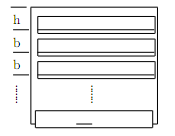
\includegraphics{./graphics/heightofpagebox.jpg}
\end{figure}
\end{comment}

\subsection{Dead cycles.} An execution of the OTR without shipping any material is called a \emph{dead cycle}. Dead cycles, have their uses and we will explain this a bit later on. However, long iterations that just return \textit{dead cycles} is an indication of an error somewhere. \tex counts the number of dead cycles in a counter named |\deadcycles| and stops the run if |\deadcycles >= \maxdeadcycles|.  In the \textit{plain} format |\maxdeadcycles| is set as 25 and in \latex as \the\deadcycles. |\maxdeadcycles = 100| is \the\maxdeadcycles. Each time |\shipout| is invoked, it resets |\deadcycles| to zero.

\begin{dispListing}
If the file is not included, reset \deadcycles, so that a long list of non-included
files does not generate an `Output loop' error.
115 \deadcycles\z@
116 \@nameuse{cp@#1}%
117 \fi
118 \let\@auxout\@mainaux}
\end{dispListing}


\subsection{\tex's Page Number.} The page number can come from any source. Salomon provides an example where the \textsc{OTR} typesets a page number from a |\count| variable. This is typeset centered below the printed area.

%\newpage
%
%Test
%\makeatletter
%
%\let\ltxxoutput\output
%\let\ltxlabel\label@name
%\output={{\let\label@name\@gobble
%  \shipout\vbox{
%  \box255\smallskip
%  \centerline{\thepage}}}
%}
%
%\vfill \penalty-10000
%
%\global\let\output\ltxxoutput
%\let\label@name\ltxlabel
%
%
%\makeatother


Notice that the output macro, just passes the contents of the box to |\shipout|. This is not actually a very good method, but is shown here to illustrate a point.

Note the |\tenrm| in the preceding example. It
is necessary because of the asynchronous nature of
the \otr. When the \otr is invoked, \tex can be
anywhere on the next page. Specifically, it could
be inside a group where a different font is used.
Without the |\tenrm|, that font (the current font)
would be used in the otr.
In the plain format, the |\count0| variable
serves as the page number, and the following two
macros are especially useful.




\subsection{The \texttt{\textbackslash vsplit} operation.} 

Supposed you have inserted the material required to go on a page on a big |\vbox|, but the material is a bit extra that what is required to fill a page exactly. You would need an operation to split the box in two. The |vsplit| operation does that. It is important to the understanding of OTR operations to have an intimate knowledge of |\vsplit|. Its syntax is: 

\begin{quote}
|\vsplit|\meta{box number} to \meta{dim}
\end{quote}

The result of the operation is a box. Most often it appears in an assignment such as: 

\begin{quote}
|\setbox1=\vsplit0 to2.6in| 
\end{quote}

This sets |\box1| to a
height of 2.6in, moves material from the top of
|\box0| to |\box1|, and keeps the remainder in |\box0|.

\begin{macro}{\loremlines}
It is important to remember that most of \tex's commands work with \latex as well. In Example~\ref{ex:loremlines}, we define a box to hold |lipsum| text in a two column layout. We want to define a macro that can split the box in as many lines as we require. 
\end{macro}

\begin{texexample}{Splitting a vbox}{ex:loremlines}
\newbox\one
\newbox\two
\long\gdef\loremlines#1#2{%
   \setbox\one=\vbox {#2}
   \setbox\two=\vsplit\one to #1\baselineskip
   \unvbox\two
   \gdef\boxone{#2}
}
\begin{multicols}{2}
\small
\loremlines{16}{\onepar}
\end{multicols}
\boxone

\setbox\one=\vbox{100}
\the\ht\one \\
\the\baselineskip
\the\splittopskip

\end{texexample}


\tex assumes that the new |\box1| may have to
be shipped out as part of the page. It therefore
places a glue similar to $h$ at the top of |\box1|.
This glue is called \docAuxCommand{splittopskip} and has a plain
format value of 10pt [348].

One important thing to note is that a box can only be split \textit{between} lines of text. 
If we split a box to another size, |\box1| will come out underfull.

Here is an \otr which splits the page, ships
out the top part and returns the rest to the MVL
(actually, to the recent contributions):

\begin{teXXX}
\output={\setbox0=\vsplit255 to1in
\shipout\box0 \unvbox255}
\end{teXXX}






\section{Communicating with the OTR: Marks}


The user can pass information to the output routine through \textit{marks}. Marks have the syntax

\begin{teX}
\mark{mark text}
\end{teX}

which is put in a mark item on the current vertical list. The mark text is subject to expansion
as in \cs{edef}.
If the mark is given in horizontal mode it migrates to the surrounding vertical lists like an
insertion item (see page Text By Topic 77); however, if this is not the external vertical list, the output routine
will not find the mark.

Marks are the main mechanism through which the output routine can obtain information
about the contents of the currently broken-off page, in particular its top and bottom. TEX sets
three variables:

{\obeylines
\cs{botmark} the last mark occurring on the current page;
\cs{firstmark} the first mark occurring on the current page;
\cs{topmark} the last mark of the previous page, that is, the value of \cs{botmark} on the previous
page.
}



If no marks have occurred yet, all three are empty; if no marks occured on the current page, all three variables are equal to the \cs{botmark} of the previous page. 

Marks can be used to get a section heading into the headline or footline of the page.

\begin{quote}
\begin{verbatim}
\def\section#1{ ... \mark{#1} ... }
\def\rightheadline{\hbox to \hsize
    {\headlinefont \botmark\hfil\pagenumber}}
\def\leftheadline{\hbox to \hsize
   {\headlinefont \pagenumber\hfil\firstmark}}
\end{verbatim}
\end{quote}

This places the title of the first section that starts on a left page in the left
headline, and the title of the last section that starts on the right page in
the right headline. Placing the headlines on the page is the job of the output
routine; see below.

It is important that no page breaks can occur in between the mark and the
box that places the title:

\emphasis{mark,nobreak}
\begin{teXXX}
\def\section#1{ ...
   \penalty\beforesectionpenalty
   \mark{#1}
   \hbox{ ... #1 ...}
   \nobreak
   \vskip\aftersectionskip
   \noindent}
\end{teXXX}

%%%%%%%%%%%% macro to put TeX references in right margin %%%%%%%% 
\newdimen\theight 
\def \TeXref#1{% 
             \vadjust{\setbox0=\hbox{\sevenrm\quad\quad\TeX book: #1}% 
             \theight=\ht0 
             \advance\theight by \dp0    \advance\theight by \lineskip 
             \kern -\theight \vbox to \theight{\rightline{\rlap{\box0}}% 
             \vss}% 
             }}% 
%%%%%%%%%%%%%%%%%%%%%%%%%%%%%%%%%%%%%%%%%%%%%%%%%%%%%%%%%%%%%%%%%%%%%%%%% 
 
However, useful these marks, sometimes an output routine (such as those found in \latexe needs to know why it was invoked. Knuth discusses in the \TeXref{396}  another method
that involves the value of the |\outputpenalty|. 
By testing for this value, it is possible to see what penalty occurred at a breakpoint;
any penalty of −10000, −10001, −10002, or less, forces the output routine to
act, hence different penalty values can be used to pass different messages. (When
the output routine puts material back on the list of contributions, it need not restore
the penalty at the breakpoint.) If output has been forced by a highly negative value
of |\outputpenalty|, the output routine can use |\vbox{\unvcopy255}| to discover how
full the page-so-far actually is. Underfull and overfull boxes are not reported when
|\box255| is packaged for use by the output routine, so there’s no harm in ejecting a
page prematurely if you want to pass a signal. (Set |\holdinginserts| positive to pass
a signal when the contents of |\box255| will be sent back through the page builder again,
if any insertions are present.)

Knuth also suggested another method that he called the \emph{dirtiest trick of all} that uses the depth 
of |\box255|. 

\section{Insertions}
Insertions are considered one of  the most  complex  topics in \tex. Many users master  topics  such 
as tokens,  file  I/O, macros,  and  even  OTRS  before they dare  tackle  insertions.  The  reason  is  that 
insertions  are  complex,  and  The \texbook, while 
covering all the relevant material, is somewhat cryptic regarding  insertions, and  lacks  simple examples. 
The  main  discussion  of  insertions takes  place  on 
[115-1251.  where \tex' s  registers  are also discussed. 
Examples  of  insertions are  shown, mostly  without 
explanations,  on  [363-364,  423-424].  A lot of what is described here is based on an article in TUGboat by David Salomon\footnote{\protect\url{http://www.tug.org/TUGboat/Articles/tb11-4/tb30salomon.pdf}}

Many users understand the idea of floats. Certain material to be typeset needs to be held in a buffer and inserted at different points on a page, for example a a figure that does not fit on a page it has to be inserted at the top of the next page. An \textit{insertion} is just a piece of a document that is generated at a certain point but appears at another point. Common examples are figures, footnotes and endnotes. Quoting Knuth:

\begin{quote}
  This  algorithm  is  admittedly  complicated, 
but  no  simpler  mechanism  seems  to  do  nearly 
as  much.
\end{quote}

\section{\protect\textbackslash shipout}

The primitive control sequence \docAuxCommand{shipout} is \tex's end game. It's syntax is quite simple:

\begin{quote}
|\shipout<box>|
\end{quote}

From TeXbook, Chapter 23: Output Routines, page 254:

\begin{quotation}
TeX’s primitive command |\shipout<box>| is what actually causes output. It sends the contents of the box to the dvi file, which is TeX’s main output file; after TeX has finished, the dvi file will contain a compact device-independent encoding of instructions that specify exactly what should be printed. When a box is shipped out, TeX displays the values of |\count0| through |\count9| on your terminal, as explained in Chapter 15; these ten counters are also recorded in the dvi file, where they can be used to identify the page. All of the |\openout, \closeout|, and |\write| commands that appear inside of the box are performed in their natural order as that box is being shipped out. Since a |\write| command expands macros, as explained in Chapter 21, TeX’s scanning mechanism might detect syntax errors while a |\shipout| is in progress. If  |\tracingoutput| is nonzero at the time of a \cs{shipout}, the contents of the box being shipped are written into your log file in symbolic form. You can say \cs{shipout} anywhere, not only in an output routine.
\end{quotation}


We can say:

\emphasize{shipout,vbox}
\begin{teXXX}
\shipout\vbox{%
  \hrule
  \medskip
  \lipsum[1-5]
  \medskip
  
  This is a Test for shipout
  
  \hrule
}
\end{teXXX}

\shipout\vbox{%
  \hrule
  \medskip
  \lipsum[1-5]
  \medskip
  \centering
  \textbf{Sample: }{This is a Test for shipout}
  \hrule
}

Since the output box handled by \tex still holds material the page is shown in the previous page. There is no page numbers or headers and it just shows he lorem-ipsum text and a primitive caption at the bottom. I have written the example to show the difference between the logical and actual pages. TeX does not care how the page will look, it will assemble it put headers, page numbers and pass it on to shipout. Shipout will then insert it to the dvi file, which will hold all teh instructions to print a real page.

We can modify the example to add our head and foot. 

\begin{texcode}{Shipout}{ex:ship2}
This will print by the normal routine

\long\gdef\boxit#1#2{\hbox{\vrule \vbox{\hrule\kern#2pt\hbox{%
\kern#2pt\vbox{#1}\kern#2pt}\kern#2pt\hrule}\vrule}}

\makeatletter
\shipout\vbox {%
  \vskip\topsep\relax
  \vskip\headsep
   \@thehead
   \vskip30pt
    \boxit{
      \lipsum[1-5]
      }{2}
   \vskip30pt
   \@thefoot   
}
\makeatother 
\end{texcode}

\latexe's output routine takes care of all the page geometry, the details to set up the headers and footers, but most importantly intercepts teh contents of the output box measure it, cuts it inserts the inserts such as footnotes and figures, margin notes, separates the text in two columns if necessary and so on. 

\long\gdef\boxit#1#2{\hbox{\vrule \vbox{\hrule\kern#2pt\hbox{%
\kern#2pt\vbox{#1}\kern#2pt}\kern#2pt\hrule}\vrule}}
\makeatletter
\shipout\vbox {%
  \vskip\topsep\relax
  \vskip\headsep
   \@thehead
   \vskip30pt
    \boxit{
      \lipsum[1-5]
      }{2}
   \vskip30pt
   \@thefoot   
}
\makeatother 



An output routine will prepare the virtual page and pass it onto a 

Here is an OTR for a \textit{framed} page. It surrounds the
page with double rules on all sides, and centers the
page number below the double box. Note that the
page shipped out is wider and taller than \cs{box255}.
The value of \cs{hsize} in this case is, therefore, not
the width of the final page shipped out, but the
width of the text lines in \cs{box255}.

Macro \cs{frameit} typesets text and surrounds it
with 4 rules (see [Ex. 21.3]). Parameter \#2 is the
space between the rules and the text. \#1 is a box
containing the text.

\emphasis{output,shipout}
\begin{texcode}{Example of simple output routine}{ex:output1}
\def\frameit#1#2{%
 \vbox{\hrule
  \hbox{%
    \vrule \kern#2pt
      \vbox{\kern#2pt #1
         \kern#2pt}%
      \kern#2pt\vrule}
\hrule}}

\output={
   \shipout\vbox{
   \boxit{\frameit{\box255}9}
      \medskip
      \centerline{Test Framed Page}}
  \advancepageno}
\end{texcode}

 

So far we did not care if the height of the page is right or not. In production code the shipout holds
a box, which has been produced by \tex. Any material we add to it, must not affect the dimensions of the box.
If we do and is too big the drivers will probably clip it.


Plain TeX has an output routine that takes care of  simple things like page numbering and insertions
using \cs{footnote} and \cs{topinsert}. 


So far we have examined the \tex OTR in detail. I hope it has given you enough understanding, not only to write your own output routine, but also to now be ready to study the \latex output routine, which is much more complicated. We have so far seen that  when \tex 
is typesetting pages of continuous text, it will gather material until it can find a least-cost page break intended to
make the gathered material fit the \cs{pagegoal} size. The
gathered material will then be placed into |\box255| and
the output routine stored in the token register \cs{output}
will be processed in a group of its own. 

Usually it will
arrange the gathered material in some way, add headers,
footlines and page numbers, and ship the gathered results out in typeset form with the \cs{shipout} command.
At the time of the \cs{shipout} command all \cs{open} and
\cs{write} commands stored in the box shipped out are expanded and written out. This is what makes it possible to have page labels corresponding to the actual page
numbers at the time of shipout: the corresponding info
is written to the |.aux| file at that time.
The output routine may decide to place material
back on the main vertical list instead of shipping it out. Its ob is to check if it can have a break, if it can it will ship the page out. If it cannot it will palce the material back on the main vertical list. 

\section{\LaTeX\  output routines}


\LaTeX\ output routine is described in \texttt{ltoutput.dtx}. You should also have a look at \texttt{ltfloat.dtx}. The algorithm is revisited i \latex3 and Frank Mittelbach, published a paper
\footnote{\protect\url{http://www.latex-project.org/papers/xo-pfloat.pdf}} in which he explains some of the problems facing the team, when dealing with the output routine.


Information on the output routine is rather scarce. Best source is a series of  articles in the TUGBoat by David Salomon.

\href{http://www.tug.org/TUGboat/Articles/tb11-1/tb27salomon.pdf}{Output Routines: Examples and Techniques. Part I: Introduction and Examples.}

\href{http://www.tug.org/TUGboat/Articles/tb11-2/tb28salomon.pdf}{Output Routines: Examples and Techniques. Part II: OTR Techniques}

\href{http://www.tug.org/TUGboat/Articles/tb11-4/tb30salomon.pdf}{Output Routines: Examples and Techniques. 
Part III: Insertions}

\href{http://www.tug.org/TUGboat/Articles/tb15-1/tb42salomon-output.pdf}{Output routines: Examples and techniques Part IV: Horizontal techniques}


David Kastrup's article \href{http://www.tug.org/TUGboat/Articles/tb24-3/kastrup.pdf}{Output Routine Requirements for Advanced Typesetting Tasks} (Proceedings of EuroTEX 2003) otlined some of the difficult areas and specifications for generic routines

The standard blocks are well described above and most tasks could be accomplished 
by rather working from
standard building blocks like \textit{insertion lists}, \textit{here points},
default mechanisms for \textit{margin notes} and so on.


%\section{Calling the output routine}
%
%The output routine is called either by TeX's normal page-breaking
%mechanism, or by a macro putting a penalty < or = -10000 in the output
%list. In the latter case, the penalty indicates why the output
%routine was called, using the following code.
%penalty reason
%
%\begin{longtable}{ll}
%\toprule
%penalty &reason\\
%\midrule
%-10000  &\ pagebreak\\
%~       &\ newpage\\
%-10001  &clearpage (\ penalty -10000 \ vbox{}| \ penalty -10001)|\\
%-10002  &float insertion, called from horizontal mode\\
%-10003 &float insertion, called from vertical mode.\\
%-10004 &float insertion.\\
%\bottomrule
%\end{longtable}
%\medskip
%
%Note: A |float| or |marginpar| puts the following sequence in the output
%list: 
%
%\begin{enumerate}
%\item a penalty of -10004,
%
%\item a null |\vbox|
%
%\item a penalty of -10002 or -10003.
%\end{enumerate}
%
%This solves two special problems:
%
%\begin{enumerate}
%\item If the float comes right after a |\newpage| or |\clearpage|,
%then the first penalty is ignored, but the second one
%invokes the output routine.
%
%\item If there is a split footnote on the page, the second 'page'
%puts out the rest of the footnote
%\end{enumerate}
%
%\latex first defines some helper routines and increase the \cs{maxdeadcycles}. The helper macros are for
%manipulating lisst.
%
%\begin{teX}
% \maxdeadcycles = 100
% \let\@elt\relax
% \def\@next#1#2#3#4{\ifx#2\@empty #4\else
%   \expandafter\@xnext #2\@@#1#2#3\fi}
%   \@next \CS \LIST {NONEMPTY}{EMPTY} == %% NOTE: ASSUME
%\@elt = \relax
% BEGIN assume that \LIST == \@elt \B1 ... \@elt \Bn
% if n = 0
% then EMPTY
% else 
%   \CS :=L \B1
%   \LIST :=G \@elt \B2 ... \@elt \Bn
%   NONEMPTY
% fi
%END
%\end{teX}
%
%
%\begin{teX}
%11 \def\@xnext \@elt #1#2\@@#3#4{\def#3{#1}\gdef#4{#2}}
%
%12 \def\@testfalse{\global\let\if@test\iffalse}
%13 \def\@testtrue {\global\let\if@test\iftrue}
%14 \@testfalse}
%   }
%
%15 \def\@bitor#1#2{\@testfalse {\let\@elt\@xbitor
%16   \@tempcnta #1\relax #2}}
%
%17 \def\@xbitor #1{\@tempcntb \count#1
%18    \ifnum \@tempcnta =\z@
%19    \else
%20      \divide\@tempcntb\@tempcnta
%21    \ifodd\@tempcntb \@testtrue\fi
%22   \fi}
%\end{teX}
%
%
%\subsection{Float boxes and lists.} 
%A \textit{float list} consisting of the 
%floats in boxes |\boxa ... \boxN| has
%the form:
%
%|\@elt \boxa ... \@elt \boxN|
%where |\boxI| is defined by
%
%|\newinsert\boxI|
%
%Normally, |\@elt| is |\let| to |\relax|. A test can be performed on the
%entire 
%oat list by locally |\def|'ing |\@elt| appropriately and
%executing the list.
%This is a lot more efficient than looping through the list.
%\LaTeX\ defines float boxes as |bx@A| to |bx@R| to make them available for 
%inserts. These will be used later to define the lists that hold these boxes. 
%
%\latex now defines the float boxes. Each one is defined as an \cmd{\newinsert.}
%
%\begin{teXXX}
%\newinsert\bx@A
%...
%\newinsert\bx@I
%\newinsert\bx@J
%\newinsert\bx@K
%\newinsert\bx@L
%\newinsert\bx@M
%\newinsert\bx@N
%\newinsert\bx@O
%\newinsert\bx@P
%\newinsert\bx@Q
%\newinsert\bx@R
%\end{teXXX}
%
%
%
%Once these boxes are defined they are inserted in the |@freelist|. At this point all the other lists are defined.
%
%\emphasis{@freelist,@toplist,@botlist,@midlist,@currlist}
%\begin{teXXX}
%41 \gdef\@freelist{\@elt\bx@A\@elt\bx@B\@elt\bx@C\@elt\bx@D
%         \@elt\bx@E
%42                 \@elt\bx@F\@elt\bx@G\@elt\bx@H\@elt\bx@I\@elt\bx@J
%43                 \@elt\bx@K\@elt\bx@L\@elt\bx@M\@elt\bx@N
%44                 \@elt\bx@O\@elt\bx@P\@elt\bx@Q\@elt\bx@R}
%\end{teXXX}
%
%\startlineat{45}
%All the lists are defined initially to be empty.
%\begin{teXXX}
%45 \gdef\@toplist{}
%46 \gdef\@botlist{}
%47 \gdef\@midlist{}
%48 \gdef\@currlist{}
%49 \gdef\@deferlist{}
%50 \gdef\@dbltoplist{}
%51 \gdef\@dbldeferlist{}
%\end{teXXX}
%
%
%The lists are similar to those defined in \texttt{plain}.
%
%\begin{description}
%\item[\cs{@freelist}] : List of empty boxes for placing new 
%floats.
%\item[\string\@toplist] : List of 
%floats to go at top of current column.
%\item[\string\@midlist] : List of 
%floats in middle of current column.
%\item[\string\@botlist] : List of 
%floats to go at bottom of current column.
%\item[\string\@deferlist] : List of 
%floats to go after current column.
%\item[\string\@dbltoplist] : List of double-col. 
%floats to go at top of current
%page.
%\item[\string\@dbldeferlist] : List of double-column 
%floats to go on subsequent
%pages.
%
%\end{description}
%
%\begin{multicols}{2}
%Check was prudent when defining the newinsert boxes in order to reserve space and memory. The package \docpkg{morefloats} can be used to add more floats to this list. This should have definitely been included here in a revision.
%
%\subsection{Defining Layout parameters} All the page layout parameters are defined next. 
%
%\begin{teXXX}
%52 \newdimen\topmargin
%53 \newdimen\oddsidemargin
%54 \newdimen\evensidemargin
%55 \let\@themargin=\oddsidemargin
%56 \newdimen\headheight
%57 \newdimen\headsep
%58 \newdimen\footskip
%59 \newdimen\textheight
%60 \newdimen\textwidth
%61 \newdimen\columnwidth
%62 \newdimen\columnsep
%63 \newdimen\columnseprule
%64 \newdimen\marginparwidth
%65 \newdimen\marginparsep
%66 \newdimen\marginparpush
%\end{teXXX}
%
%Remember  that TeX knows little about a page. The problem is that TEX has no idea how
%wide and tall the paper is. All it knows is the
%left and top offsets, and the dimensions of the
%printed area (|\hsize| and |\vsize|). All these dimensions need to be calculated and adjustments made within the \otr.
%
%A document normally  starts by specifying:
%
%\begin{teXXX}
%\newdimen\paperheight
%\newdimen\paperwidth
%\paperheight=..in \paperwidth=..in
%\end{teXXX}
%
%
%\end{multicols}
%
%
%\subsection*{The AtBeginDvi}
%A box register is used  to put stuff that must appear before anything else
%in the |.dvi| file.
%
%The stuff in the box should not add any typeset material to the page when it
%is unboxed.
%
%\emphasis{AtBeginDvi,@begindvibox}
%
%\begin{teXXX}
%67 \newbox\@begindvibox
%68 \def \AtBeginDvi #1{%
%69 \global \setbox \@begindvibox
%70 \vbox{\unvbox \@begindvibox #1}%
%71 }
%\end{teXXX}
%
%\begin{teXXX}
%72 \newdimen\@maxdepth
%73 \@maxdepth = \maxdepth
%\end{teXXX}
%
%
%Some new registers for paperheight and paperwidth are defined:
%
%\begin{teXXX}
%74 \newdimen\paperheight
%75 \newdimen\paperwidth
%76 \newif \if@insert
%These should definitely be global:
%77 \newif \if@fcolmade
%78 \newif \if@specialpage \@specialpagefalse
%These should be global but are not always set globally in other les.
%79 \newif \if@firstcolumn \@firstcolumntrue
%80 \newif \if@twocolumn \@twocolumnfalse
%Not sure about these: two questions. Should things which must apply to a whole
%doument be local or global (they probably should be `preamble only' commands)?
%Are these three such things?
%81 \newif \if@twoside \@twosidefalse
%82 \newif \if@reversemargin \@reversemarginfalse
%83 \newif \if@mparswitch \@mparswitchfalse
%This counter has been imported from `multicol'.
%84 \newcount \col@number
%85 \col@number \@ne
%\end{teXXX}
%
%and a lot of other internal registers
%
%\begin{teX}
%86 \newcount\@topnum
%87 \newdimen\@toproom
%88 \newcount\@dbltopnum
%89 \newdimen\@dbltoproom
%90 \newcount\@botnum
%91 \newdimen\@botroom
%92 \newcount\@colnum
%93 \newdimen\@textmin
%94 \newdimen\@fpmin
%95 \newdimen\@colht
%96 \newdimen\@colroom
%97 \newdimen\@pageht
%98 \newdimen\@pagedp
%99 \newdimen\@mparbottom \@mparbottom\z@
%100 \newcount\@currtype
%101 \newbox\@outputbox
%102 \newbox\@leftcolumn
%103 \newbox\@holdpg
%104 \def\@thehead{\@oddhead} % initialization
%105 \def\@thefoot{\@oddfoot}
%\end{teX}
%
%
%\subsection{\texttt{\textbackslash clearpage}}
%
%\begin{macro}{\clearpage}
%The clearpage macro is a bit complicated, as it needs to avoid a complete empty page after a |\twocolumn[..]|. This prevents the text from the argument
%vanishing into a  float box, never to be seen again. We hope that it does not
%produce wrong formatting in other cases.
%\end{macro}
%
%\begin{teXXX}
%106 \def\clearpage{%
%107   \ifvmode
%108   \ifnum \@dbltopnum =\m@ne
%109     \ifdim \pagetotal <\topskip
%110       \hbox{}%
%111     \fi
%112   \fi
%113  \fi
%114 \newpage
%115 \write\m@ne{}%
%116 \vbox{}%
%117 \penalty -\@Mi
%118 }
%\end{teXXX}
%
%\subsection{The \texttt{\textbackslash clearpagedoublepage} macro} 
%
%\begin{macro}{cleardoublepage}
%This checks for odd and even pages by using the
%page counter |c@page|.  It also provides switches of twoside printing. 
%
%\numberlineat{119}
%\begin{teXXX}
%\def\cleardoublepage{%
%   \clearpage
%   \if@twoside 
%     \ifodd\c@page
%     \else
%       \hbox{}
%       \newpage
%       \if@twocolumn\hbox{}\newpage
%       \fi
%     \fi
%  \fi}
%\end{teXXX}
%\end{macro}
%
%Note the |\newpage| is defined a bit further on. This is a fairly simple definition, since most of the code that follows only gets a bit complicated with the twocolumn option. It sets the dimensions and the booleans to those appropriate for the |onecolumn| option. An important note we back to \tex's |\hsize|. Both the linewidth as well as the columnwidth are set to this.
%
%\begin{teXXX}
%123 \def\onecolumn{%
%124   \clearpage
%125   \global\columnwidth\textwidth
%126   \global\hsize\columnwidth
%127   \global\linewidth\columnwidth
%128   \global\@twocolumnfalse
%129   \col@number \@ne
%130   \@floatplacement
%     }
%\end{teXXX}
%
%\subsection{\string newpage.} 
%
%The |\newpage| macro is programmed defensively. The two checks at the beginning ensure that an item label or run-in section title
%immediately before a |\newpage| get printed on the correct page, the one before
%the page break.
%All three tests are largely to make error processing more robust; that is why
%they all reset the 
%flags explicitly, even when it would appear that this would be
%done by a |\leavevmode|.
%
%\begin{teXXX}
%131 \def \newpage {%
%132  \if@noskipsec
%133    \ifx \@nodocument\relax
%134      \leavevmode
%135      \global \@noskipsecfalse
%136    \fi
%137 \fi
%138 \if@inlabel
%139   \leavevmode
%140   \global \@inlabelfalse
%141 \fi
%142 \if@nobreak \@nobreakfalse \everypar{}\fi
%143 \par
%144 \vfil
%145 \penalty -\@M}
%\end{teXXX}
%
%An empty cols is defined. There is a note here, that an invisible rule might have been a better idea.
%
%\begin{teXXX}
%146 \def \@emptycol {\vbox{}\penalty -\@M}
%\end{teXXX}
%
%\subsection{The \string twocolumn macro.} This is the longest definition so far. We will leave it for a while and then come back. There are several bug fixes to the two-column stuff here. Firstly, like the onecolumn the page parameters are set to the correct parameters.
%
%
%\begin{teXXX}
%147 \def \twocolumn {%
%148 \clearpage
%149 \global\columnwidth\textwidth
%150 \global\advance\columnwidth-\columnsep
%151 \global\divide\columnwidth\tw@
%152 \global\hsize\columnwidth
%153 \global\linewidth\columnwidth
%154 \global\@twocolumntrue
%155 \global\@firstcolumntrue
%156 \col@number \tw@
%\end{teXXX}
%
%
%
%\section{The output macro}
%
%The setting of the \cs{output} is quite short but it belies its complexity.
%After having checked verious parameters it redirects to |@specialoutput|. This is the heart of the routines. Notice that \latex just fills in the token list of \tex's |output| routine, it does not attempt to redefine it or save it. 
%Should some hooks be defined here, life might have been made easier, however, what one can do is to first save the \latex output routine and then redefine the output as one may wish. Return to it can happen after it. If you take this approach, you should be careful of packages that redefine output, such as |multicol| and |longtable|. An approach such as this is taken by \citeauthor{revtex} in the \pkgname{revtex} class.\footcite[][This is a document class of the American Physical Society. It enables submission to any of the APS journals. Its distribution point is \protect\url{http://publish.aps.org/revtex4/}]{revtex}
%
%\emphasis{ifnum,fi,else,ifdimen,@specialoutput}
%\begin{teX}
%204 \output {%
%205 \let \par \@@par
%206 \ifnum \outputpenalty<-\@M
%207    \@specialoutput
%208 \else
%209    \@makecol
%210    \@opcol
%211    \@startcolumn
%212    \@whilesw \if@fcolmade \fi
%213      {%
%218      \@opcol\@startcolumn}%
%219 \fi
%220 \ifnum \outputpenalty>-\@Miv
%221 \ifdim \@colroom<1.5\baselineskip
%222 \ifdim \@colroom<\textheight
%223 \@latex@warning@no@line {Text page \thepage\space
%224 contains only floats}%
%225 \@emptycol
%226 % \if@twocolumn
%227 % \if@firstcolumn
%228 % \else
%229 % \@emptycol
%230 % \fi
%231 % \fi
%232 \else
%  233 \global \vsize \@colroom
%234 \fi
%235 \else
%236   \global \vsize \@colroom
%237 \fi
%238 \else
%239   \global \vsize \maxdimen
%240 \fi
%241 }
%\end{teX}
%
%
%
%\begin{teXXX}
%244 \gdef\@specialoutput{%
%245   \ifnum \outputpenalty>-\@Mii
%246     \@doclearpage
%247   \else
%248     \ifnum \outputpenalty<-\@Miii
%249         \ifnum \outputpenalty<-\@MM \deadcycles \z@ \fi
%250                 \global \setbox\@holdpg \vbox {\unvbox\@cclv}%
%251         \else
%252         \global \setbox\@holdpg \vbox{%
%253                 \unvbox\@holdpg
%254                 \unvbox\@cclv
%We must now remove the box added by the 
%oat mechanism and the \topskip
%glue therefore added above it by TEX.
%255                \setbox\@tempboxa \lastbox
%256                \unskip
%257 }%
%These two are needed as separate dimensions only by \@addmarginpar; for other
%purposes we put the whole size into \@pageht (see below).
%258                \@pagedp \dp\@holdpg
%259                \@pageht \ht\@holdpg
%260                \unvbox \@holdpg
%
%261                \@next\@currbox\@currlist{%
%262                \ifnum \count\@currbox>\z@
%Putting the whole size into \@pageht (see above).
%263                  \advance \@pageht \@pagedp
%264                  \ifvoid\footins \else
%265                    \advance \@pageht \ht\footins
%266                    \advance \@pageht \skip\footins
%267                    \advance \@pageht \dp\footins
%268                \fi
%\end{teXXX}
%
%
%
%\subsection{The \string @doclearpage macro.} This is an emergency action. It dumps everything: footnotes first and then floats. 
%
%
%\section*{The Kludgeins}
%
%The kludgeins are simply inserts that fool \tex in enlarging a page by a small amount, normally used to allow one or two lines of text to go in the same page.
%
%The two kludgeins mentioned in the kernel are are \cs{enlargethisspace} and its star version.\footnote{The Oxford English Dictionary (2nd ed., 1989) kludge entry cites one source for this word's earliest recorded usage, definition, and etymology: Jackson W. Granholm's 1962 "How to Design a Kludge" article, which appeared in the American computer magazine Datamation
%kludge  Also kluge. [J. W. Granholm's jocular invention: see first quot.; cf. also bodge v., fudge v.]
%
%'An ill-assorted collection of poorly-matching parts, forming a distressing whole' (Granholm); esp. in Computing, a machine, system, or program that has been improvised or 'bodged' together; a hastily improvised and poorly thought-out solution to a fault or 'bug'.
%
%The word 'kludge' is...derived from the same root as the German Kluge..., originally meaning 'smart' or 'witty'.... 'Kludge' eventually came to mean 'not so smart' or 'pretty ridiculous'.}
%
%
%
%\begin{teXX}
%\gdef \enlargethispage{%
%1198 \@ifstar
%1199 {%
%1203   \@enlargepage{\hbox{\kern\p@}}}%
%1204 {%
%1208   \@enlargepage\@empty}%
%1209 }
%\end{teXX}
%
%Adds |<dim>| to the height of the current column only. On the printed page the
%bottom of this column is extended downwards by exactly |<dim>| without having
%any effect on the placement of the footer; this may result in an overprinting.
%\cs{enlargethispage}.
%
%Similar to |\enlargethispage| but it tries to squeeze the column to be printed
%in as small a space as possible, ie it uses any shrinkability in the column. If the
%column was not explicitly broken (e.g. with |\pagebreak|) this may result in an
%overfull box message but except for this it will come out as expected (if you know
%what to expect).
%The star form of this command is dedicated to Leslie Lamport, the other we
%need for ourselves (FMi, CAR).
%These commands may well have unwanted if used soon before a\ldots
%
% 




\section{Packages}

OTR routines are notoriously difficult to debug and define. Some of the available packages at CTAN
can make the programming job easier.

The \pkg{everypage} package by Sergio Callegari provides hooks into the \latex\ internal commands to
to do actions on every page or on the current page. Specifically, actions  are performed \emph{before} the page is shipped, so they can be used to put watermarks \emph{in the background} of a page, or to
set the page layout. 

The package provides two hooks:

\emphasis{AddEverypageHook,AddThisPageHook}
\begin{teXXX}
  \AddEverypageHook{Test}
  \AddThisPageHook
\end{teXXX}

The package reminds in some sense
\pkgname{bobhook} by Karsten Tinnefeld, but it differs in the way in
 which the hooks are implemented, as detailed in the following.
 In some sense it may also be related to the package
 \pkgname{everyshi} by Martin Schroeder, but again the implementation
 is different.

 
 This program adds two \LaTeX\ hooks that get run when document
 pages are finalized and output to the |.dvi| or |.pdf|
 file. Specifically, one hook gets executed on every page, while the
 other is executed for the current page. Hook actions are are performed
 \emph{before} the page is output on the medium, and this is
 important to be able to play with the page layout or to put things
 \emph{behind} the page contents (e.g., watermarks such as an image,
 framing, the ``DRAFT'' word, and the like).
 
 The package reminds in some sense \pkg{bobhook} by Karsten
 Tinnefeld, but it differs in the way in which the hooks are
 implemented:
 


 \begin{enumerate}
 \item there is no formatting inherent in the hooks. If one wants to
   put some watermark on a page, it is his own duty to put in the
   hook the code to place the watermark in the right position. Also
   note that the hooks code should \emph{eat up no space} in the
   page.  Again, if the hooks are meant to place some material on the
   page, it is the duty of the hook programmer to put code in the
   hooks to pretend that the material has zero width and zero height.
   The implementation is \emph{lighter} than the \Lpack{bobhook} one,
   and possibly more flexible, since one is not limited by any
   pre-coded formatting for the hooks. On the other hand it is
   possibly more difficult to use. Nonetheless, it is easy to think
   of other packages relying on \Lpack{everypage} to deliver more
   user-friendly and \emph{task specific} interfaces. Already there
   are a couple of them: the package \Lpack{flippdf} produces
   mirrored pages in a PDF document and \Lpack{draftwatermark}
   watermarks document pages.
 \item similarly to \Lpack{bobhook} and \Lpack{watermark}, the
   package relies on the manipolatoin of the internal \LaTeX\ macro
   |\@begindvi| to do the job. However, the redefinition of
   |\@begindvi| is here postponed as much as possible, striving to
   avoid interference with other packages using |\AtBeginDvi| or
   anyway manipulating |\@begindvi|. Specifically \Lpack{everypage}
   makes no special assumption on the initial code that |\@begindvi|
   might contain.
 \end{enumerate}



Also in some sense \pkgname{everypage} can be related to package
 \pkgname{everyshi} by Martin Schr\"oeder \cite{everyshi}, but it differs radically from
 it in the implementation. In fact,\pkgname{everypage} operates by
 manipulation of the |\@begindvi| macro, rather than at the
 lower level |\shipout| macro.

\section{hooking at shipout}

\begin{docCmd} {EveryShipout} {}
\begin{docCmd} {AtNextShipout} {}
This package provides the hooks \cs{EveryShipout} and 
  \cs{AtNextShipout} whose arguments are executed after the output 
  routine has constructed \cs{box255}, and before \cs{shipout} is 
  called.
\end{docCmd}
\end{docCmd}

An example application for this package would be a package for
 adding text to the bottom of each page.
 The  \pkgname{prelim2e} package adopts this method \citep{prelim2e}.\footcite{prelim2e}

The solution  uses is based on code developed in  |quire.tex| by
 Marcel R.~van der Goot.\footcite{quire}  

The \pkgname{prelim2e}  intercepts and modifies the |\box255|. 

\begin{teX}
44 \newcommand{\@Prelim@EveryShipout}{%
45 \bgroup
% First we save the dimensions of \box255: height, width and depth; and calculate
% the total height of \box255.
46 \dimen\z@=\wd\@cclv
47 \dimen\@ne=\ht\@cclv
48 \dimen\tw@=\dp\@cclv
49 \dimen\thr@@=\dimen1
50 \advance\dimen\thr@@ by \dimen\tw@
% Then we set \box255: A \vbox to the total height of \box255. In this a \hbox to
% the width of \box255 is included, in which \box255 is set.
51 \global\setbox\@cclv\vbox to \dimen\thr@@{%
52 \hb@xt@\dimen\z@{%
53 \box\@cclv%
54 \hss
55 }%
\end{teX}
To this we append the text produced by |\PrelimText|. It is put in a |\vbox to 0pt|
in which a |\hbox| to the width of |\box255| is included, in which |\PrelimText| is set.
We have to reset |\protect| because it is set to |\noexpand| by the output routine.

\begin{teXXX}
56 \vbox to \z@{%
57   \hb@xt@\dimen\z@{%
58     \let\protect\relax
59     \hfill\PrelimText\hfill
60   }%
61   \vss
62 }%
63   \vss
64 }%
\end{teXXX}

Finally we set the dimensions of |\box255| to the values they had before |\@Prelim@EveryShipout|.

\begin{teX}
65 \wd\@cclv=\dimen\z@
66 \ht\@cclv=\dimen\@ne
67 \dp\@cclv=\dimen\tw@
68 \egroup
69}
\end{teX}

Once the command is defined, it is hooked into the system via |\EveryShipout| when it is in draft mode. 

\begin{teX}
70 \if@prelim@draft
71 \EveryShipout{\@Prelim@EveryShipout}
72 \fi
\end{teX}

\section{How to place a background image}

One can use \tikzname to place a background image or some text on a page

First we define some utility macros:


\begin{teX}
\def\bg@contents{Draft}
\def\bg@color{red!45}
\def\bg@angle{60}
\def\bg@opacity{.5}
\def\bg@scale{15}
\def\bg@position{current page.center}
\def\bg@anchor{}
\def\bg@hshift{0}
\def\bg@vshift{0}
\end{teX}

A new command is then developed to describe the background material

\begin{teXXX}
\newcommand\bg@material{%
   \begin{tikzpicture}[remember picture,overlay]
   \node [rotate=\bg@angle,scale=\bg@scale,opacity=\bg@opacity,%
   xshift=\bg@hshift,yshift=\bg@vshift,color=\bg@color]
   at (\bg@position) [\bg@anchor] {\bg@contents};
  \end{tikzpicture}}%
\end{teXXX}


Once the background material has been defined we can place it on the page by simply calling:

\begin{teX}
\newcommand\BgThispage{\AddThispageHook{\bg@material}}
\end{teX}


The \pkgname{background}\footcite{background} package by \citeauthor has capitalized on two good packages the \tikzname and the \pkgname{everypage}.
\footcite{everypage} As most of modern
\tex programming works with |pdf| files, package developers prefer to use \tikzname methods for hooking directly into the pdf and thus avoid a trip into the output routine. If it is required then it hooks via the dvi or shipout commands.\footnote{These packages are loaded automatically by the \pkgname{phd-pkgmanager}.}



\vfill

\message{(total: \the\pagetotal
depth: \the\pagedepth
shrink: \the\pageshrink
stretch: \the\pagestretch}



 







































% 
%</driver>
% \fi
% 
%  \CheckSum{0}
%  \CharacterTable
%  {Upper-case    \A\B\C\D\E\F\G\H\I\J\K\L\M\N\O\P\Q\R\S\T\U\V\W\X\Y\Z
%   Lower-case    \a\b\c\d\e\f\g\h\i\j\k\l\m\n\o\p\q\r\s\t\u\v\w\x\y\z
%   Digits        \0\1\2\3\4\5\6\7\8\9
%   Exclamation   \!     Double quote  \"     Hash (number) \#
%   Dollar        \$     Percent       \%     Ampersand     \&
%   Acute accent  \'     Left paren    \(     Right paren   \)
%   Asterisk      \*     Plus          \+     Comma         \,
%   Minus         \-     Point         \.     Solidus       \/
%   Colon         \:     Semicolon     \;     Less than     \<
%   Equals        \=     Greater than  \>     Question mark \?
%   Commercial at \@     Left bracket  \[     Backslash     \\
%   Right bracket \]     Circumflex    \^     Underscore    \_
%   Grave accent  \`     Left brace    \{     Vertical bar  \|
%   Right brace   \}     Tilde         \~}
%
%
%
% \changes{1.0}{2018/01/26}{Converted to DTX file}
%
% \DoNotIndex{\newcommand,\newenvironment}
% \GetFileInfo{phd.dtx}
% 
%  \def\fileversion{v1.0}          
%  \def\filedate{2012/03/06}
% \title{The \textsf{phd} package.
% \thanks{This
%        file (\texttt{phd-utils.dtx}) has version number \fileversion, last revised
%        \filedate.}
% }
% \author{Dr. Yiannis Lazarides \\ \url{yannislaz@gmail.com}}
% \date{\filedate}
%
%
% 
% ^^A\maketitle
% 
% ^^A\frontmatter
%  ^^A\coverpage{./images/hine02.jpg}{Book Design }{Camel Press}
%  \newpage
% ^^A\secondpage
% \pagestyle{empty}
%
% \pagestyle{headings}
% \raggedbottom
% ^^A \StopEventually{}
%  \OnlyDescription
%
%  ^^A\StopEventually{\printindex}
%<*package>
% \CodelineNumbered
% \pagestyle{headings}
% 
% \chapter{Implementation}
%
% The implementation is divided into different parts. 
% These parts are sometimes placed smaller packages 
% to make their maintenance easier and also to enable,
% partial deployment.
% 	
% \begin{description}
%
%  \item[The Package Manager] This section is responsible 
%       for pre-loading  packages, resolving conflicts and 
%       providing all interfacing commands (see \docFile{phd-pkgmanager}).
%
%
%  \item[Scripts Manager] Manages the loading of scripts for the worlds 
%  laguages and scripts.
%
%  \item[Keys] Key values are managed through \pgfname. The package
%       \pkg{phd-handlers} provides some useful handlers, mostly used by
%       internally.
%
%  \item[Epigraphs] A small supplementary package for epigraphs.
%
%  \item[MWE] The package generates a large number
%		of Minimum Working Examples that we use for testing. 
%		Most of them can also used as examples for training 
%		or self-study.
%
%  \item[Counters] The package counters, is an extension to the current
%    \latexe package offering more functionality and close integration
%    with the rest of the |phd| packages.
%
% \end{description}
%
% \section{Preliminaries}
%
%   Standard file identification. We first announce the package 
%	 and require that it be used with \LaTeX2e. RE
%
%    \begin{macrocode}
\NeedsTeXFormat{LaTeX2e}[2017/04/15]%
\ProvidesPackage{phd-utils}[2018/1/13 v1.0 various useful utilities (YL)]%
%    \end{macrocode}
%
% \section{spacing}
% {hspace} This is a \textit{hairspace}, here defined 
% as 1pt.
% {hquad} This is a half squad space
%    \begin{macrocode}
\newcommand{\hairsp}{\hspace{1pt}}% hair space
\newcommand{\hquad}{\hskip0.5em\relax}% half quad space
% Sometimes, we need a little more horizontal spacing, too (used for symbols).
\newcommand{\qqquad}{\qquad\quad}
\newcommand{\ie}{\textit{i.\hairsp{}e}\xspace} %removed\@
\newcommand{\eg}{\textit{e.\hairsp{}g.}\xspace}

\newcommand{\BC}[1]{\textsc{#1~bc}} %European Union Style Guide FIX

\newcommand{\AD}[1]{\textsc{ad~#1}} %European Union Style Guide FIX
\newcommand{\bce}[1]{\textsc{bce~#1}}
%    \end{macrocode}
% 
%
% \subsection{Standard phantom widths}
%
%    \begin{macrocode}
\newcommand\Zi{\phantom{0}} %Z conflicts with symbols 
\newcommand\ZZ{\phantom{00}}
\newcommand\ZZZ{\phantom{000}}
\newcommand\ZZZZ{\phantom{0000}}
\providecommand\newthought[1]{%
   \addvspace{1.0\baselineskip plus 0.5ex minus 0.2ex}%
   \noindent\textsc{#1}%
}
  \let\equation\gather             %% See tabu and hyperref docs
  \let\endequation\endgather
%    \end{macrocode}
% Support for quick setting of variables
%    \begin{macrocode}
\def\phddefvar#1#2{%
  \expandafter\def\csname PHDvar@#1\endcsname{#2}%
}
\def\phdifvar#1{%
  \expandafter\ifx\csname PHDvar@#1\endcsname\relax
    \expandafter\@secondoftwo
  \else
    \expandafter\@firstoftwo
  \fi
}
\def\phdusevar#1{%
  \phdifvar{#1}{%
    \csname PHDvar@#1\endcsname
  }{%
    variable #1\undefined
  }%
}
%    \end{macrocode}
% \section{Rules}
% We need to define a number of rules to use in typesetting styles.
%	We will use later on different styles of rules to decorate chapter headings.
%	We define a few here to simplify code later on.
%
%    \begin{macrocode}
\DeclareRobustCommand\thickrule{%
    \leavevmode \leaders \hrule height 2pt \hfill \kern \z@}
\DeclareRobustCommand\thinrule{\vrule width\textwidth height0.4pt depth0pt\relax}%
%
\DeclareRobustCommand\mediumrule{\rule{\textwidth}{0.8pt}}
%    Adjusted to get toc parameters in
\DeclareRobustCommand\Rule{{\color{\tocchapternumberfill@cx}\rule[-4.1pt]{13cm}{0.4pt}}}
\DeclareRobustCommand\bottomline{\medskip
   \noindent\rule{\linewidth}{0.4pt}\medskip}
\DeclareRobustCommand\topline{\par\medskip
   \noindent\rule{\linewidth}{0.4pt}\medskip} 
%    \end{macrocode}
% 
% 
% 
%
%  Some chapter and sectioning heads include rules, we define them here for convenience.
%
%    \begin{macrocode}
\cxset{chapter rule color/.store in={\chapter@rule@color}}%
\cxset{chapter rule color=spot!30}
\DeclareRobustCommand\tikzrule{%
  \tikz [color=\chapter@rule@color, very thick, inner sep=0pt, outer sep=0pt]%
        \draw(0,0)--(\the\linewidth,0);
}%
%  The trim left is required to align the rule exactly
%    \begin{macrocode}           
%#1  options #2 width  #3 height           
\newcommand\drawrule[3][]{%
    \offinterlineskip
          \tikz [ name=s,trim left,
                   anchor=base,
                   draw=black, 
                 % double distance=.2pt,
                  line width=#3,
                  %very thick,
                  inner sep=0pt, 
                  outer sep=0pt,#1]   \draw(0,0)--(#2,0);
}
 \def\drawdoublerule#1#2{%
    \drawrule{#1}{#2}%
    \vskip2.5pt
    \drawrule{#1}{#2}%
 }
%    \end{macrocode}
%
% \section{Assertions}
% some assertions
%    \begin{macrocode}
\def\TRUE{ \meta{true code} }
\def\FALSE{ \meta{false code} }
\def\PASS{\par{\bfseries\textcolor{green!50!blue}{PASS}}\ ~}
\def\FAIL{\par{\bfseries\textcolor{red!70!black}{FAIL}}\ ~}
%    \end{macrocode}
% upquote needs to be loaded before listings? Must test
% does not seem to matter actually...
%
%\iffalse
%</package>
%\fi
%
%
% \printindex
% \Finale
\endinput




